\documentclass[11pt,a4paper]{article}

\usepackage{graphicx}
\usepackage{color}
\usepackage{amsmath}
\usepackage{amssymb}
\usepackage{listings}
\usepackage{hyperref}

\lstset{language=c++}
\lstset{basicstyle=\tiny}
\lstset{backgroundcolor=\color{white}}
\lstset{frame=single}
\lstset{stringstyle=\ttfamily}
\lstset{keywordstyle=\color{red}\bfseries}
\lstset{commentstyle=\itshape\color{blue}}
\lstset{showspaces=false}
\lstset{showstringspaces=false}
\lstset{showtabs=false}
\lstset{breaklines}

\title{Solving the Eigenvalue Problem Using Jacobi's Algorithm}
\author{John Bower}
\date{February 12 2016}

\begin{document}
\maketitle

\begin{abstract}

In this project I investigate Jacobi's algorithm as a means to solve the eigenvalue problem, particularly for one and two electrons in a potential well. While the algorithm is accurate when compared with available analytical solutions, the computational time is significantly longer than freely available library functions in C++, specifically armadillo. Next, I find that the role of repulsion varies according to the strength of the potential, with more relative importance for shallower potential wells.

\end{abstract}

\begin{itemize}
\item All source files and benchmark calculations can be found at \url{https://github.com/johnbower2012/CPMSU_work/tree/master/project2}.
\item A list of all code files can be found at the end of this document.
\end{itemize}

\section{Introduction}

Since its publication ninety years ago, Schr{\"o}dinger's equation
\begin{equation}
\hat{H}\Psi = E\Psi,
\end{equation}
and the so called "quantum" realm which it describes continue to form an area of intense interest, and not merely for fundamental research. Quantum dots, for example, are electrons tightly confined within potential wells; a simple idea, yet they currently range across the field of application, from energy production in solar cell research to a more color rich and enery efficient television experience in LCD displays. Herein we provide a simple model for the quantum dot problem where the potential is harmonic. 

Schr{\"o}dinger's equation itself has often been interpreted as a differential equation, where $\hat{H}$ describes a hamiltonian with energy $E$ and respective state function $\Psi$. However, this same equation can also be interpreted as an eigenvalue problem wherein a hamiltonian has with a set of eigenvalues ${E_i}$ with respective column eigenvectors ${\hat{\psi}_i}$. Specifically,
\begin{equation}
\hat{H}\hat{\Psi} = \hat{\Lambda} = \big[E_1\hat{\psi_1} \hspace{0.1 cm} \dots \hspace{0.1 cm} E_n\hat{\psi}_n\big].
\end{equation}

In this project I begin with the former picture to shape three simple cases into eigenvalue problems. The reasons are twofold. First, we will test Jacobi's algorithm for its accuracy, speed, and stability in solving an eigenvalue problem on the case of a single electron in a harmonic potential, one of the few cases where analytical solutions are known. Second, with the case of two electrons in a harmonic potential, we will not only test the algorithm against known solutions but also test the contribution of repulsion as we vary the strength of the harmonic potential. 

\section{Theory}
We split the proceeding work into two steps, namely the formulation and simplification of the differential equations, and then the discretization of the domain such that we are able to compute numerically the resulting eigenvalue problem.

\subsection{Formulation of the Three Cases}
We begin with the single electron in a harmonic potential. 
Recalling equation (1), we expand $\hat{H}$ into its typical form,
\begin{equation}
\bigg(\frac{-\hbar^2}{2m}\nabla^2 + V(\vec{r})\bigg)\Psi(\vec{r}) = E\Psi(\vec{r}).
\end{equation}
Simplifying for three dimensions and extracting only the portion which is of interest to us, the radial piece, we have
\begin{equation}
\frac{-\hbar^2}{2m}\bigg(\frac{1}{r^2}\frac{d}{dr}r^2\frac{d}{dr} - \frac{l(l+1)}{r^2}\bigg)\psi(r) + V(r)\psi(r) = E\psi(r).
\end{equation}
Allowing $\psi(r) \rightarrow \frac{u(r)}{r}$, we arrive at a much simpler expression,
\begin{equation}
\frac{-\hbar^2}{2m}\bigg(\frac{d^2}{dr^2}u(r) - \frac{l(l+1)}{r^2}\bigg)u(r) + V(r)u(r) = Eu(r), 
\end{equation}
where we also let $r \rightarrow \rho\alpha$, $\rho$ now dimensionless, so that
\begin{equation}
\frac{-\hbar^2}{2m\alpha^2}\bigg(\frac{d^2}{d\rho^2}u(\rho) - \frac{l(l+1)}{\rho^2}\bigg)u(\rho) + V(\rho)u(\rho) = Eu(\rho).
\end{equation}
Multiplying through by $\frac{2m\alpha^2}{\hbar^2}$, we get
\begin{equation}
-\frac{d^2}{d\rho^2}u(\rho) + \bigg(\frac{l(l+1)}{\rho^2} + \frac{2m\alpha^2}{\hbar^2}V(\rho)\bigg)u(\rho) = \frac{2m\alpha^2E}{\hbar^2}u(\rho).
\end{equation}
Here we set $l = 0$ and finally input our desired harmonic potential $V(\rho)$ = $\frac{1}{2}k\alpha^2\rho^2$,
\begin{equation}
-\frac{d^2}{d\rho^2}u(\rho) + \frac{mk\alpha^4}{\hbar^2}\rho^2u(\rho) = \frac{2m\alpha^2E}{\hbar^2}u(\rho),
\end{equation}
so that we arrive at our final form,
\begin{equation}
\boxed{-u''(\rho) + \rho^2u(\rho) = \lambda u(\rho), \hspace{1.0 cm} \alpha = \bigg(\frac{\hbar^2}{mk}\bigg)^{\frac{1}{4}}, \hspace{0.5 cm} \lambda = \frac{2m\alpha^2E}{\hbar^2}}
\end{equation}

Next, we consider two electrons. Taking a queue from the one electron case, we begin straight from the radial equation for two electrons in a harmonic potential,
\begin{equation}
\bigg(-\frac{\hbar^2}{2m}\frac{d^2}{dr_1^2}u(r_1) - \frac{\hbar^2}{2m}\frac{d^2}{dr_2^2}u(r_2) + \frac{1}{2}kr_1^2 + \frac{1}{2}kr_2^2 + \frac{e^2\beta}{|\vec{r}_1 - \vec{r}_2|}\bigg)u(r_1,r_2) = E^{(2)}u(r_1,r_2),
\end{equation}
where $e^2\beta$ = 1.44 eVnm. In order to separate out the terms with which the repulsion will interact, we define new variables $\vec{r} = \vec{r}_1 - \vec{r}_2$, and $\vec{R} = \frac{1}{2}(\vec{r}_1 + \vec{r}_2)$, where $\vec{r}$ is the separation vector and $\vec{R}$ is the center of mass vector, with the result 
\begin{equation}
\bigg(-\frac{\hbar^2}{m}\frac{d^2}{dr^2} - \frac{\hbar^2}{4m}\frac{d^2}{dR^2} + \frac{1}{4}kr^2 + kR^2 + \frac{e^2\beta}{r}\bigg)u(r_1,r_2) = (E_r + E_R)u(r,R).
\end{equation}
Here we keep only the terms associated with the separation distance $r$, so that we have 
\begin{equation}
\bigg(-\frac{\hbar^2}{m}\frac{d^2}{dr^2} + \frac{1}{4}kr^2 + \frac{e^2\beta}{r}\bigg)u(r) = E_ru(r)
\end{equation}
Retracing the steps from a single electron, we define $r \rightarrow \alpha\rho$, and so
\begin{equation}
\bigg(-\frac{\hbar^2}{m\alpha^2}\frac{d^2}{d\rho^2} + \frac{1}{4}k\alpha^2\rho^2 + \frac{e^2\beta}{\alpha\rho}\bigg)u(\rho) = E_{\rho}u(\rho)
\end{equation}
Finally, we arrive at our final form for the two electron case where
\begin{equation}
-u''(\rho) + \bigg(\frac{km\alpha^4}{4\hbar^2}\rho^2 + \frac{\alpha\beta e^2m}{\hbar^2}\frac{1}{\rho}\bigg)u(\rho) = \frac{m\alpha^2E_{\rho}}{\hbar^2}u(\rho).
\end{equation}
Simplifying and condensing our equation so as to grasp the essential nature of our solution, we arrive at
\begin{equation}
\boxed{-u''(\rho) + \bigg(\omega^2\rho^2 + \frac{1}{\rho}\bigg)u(\rho) = \lambda u(\rho)}
\end{equation}
where
\begin{equation}
\boxed{\alpha = \frac{\hbar^2}{\beta e^2m}, \hspace{1.0 cm} \omega^2 = \frac{km\alpha^4}{4\hbar^2}, \hspace{1.0 cm} \lambda = \frac{m\alpha^2E_{\rho}}{\hbar^2}}
\end{equation}{
Here we see we have finally arrived at an equation where we consider the dimensionless separation distance $\rho$ between two electrons in a harmonic potential with a specific frequency $\omega$. This splits into our two cases, with and without repulsion. The one without repulsion simply drops the term $\frac{1}{\rho}$ term while the term with repulsion is given as above.

Note that each case results in a similar form, where we may simply write
\begin{equation}
-u''(\rho) + \tilde{V}(\rho)u(\rho) = \lambda u(\rho),
\end{equation}
understanding that $\tilde{V}(\rho)$ and $\lambda$ change for each case.

\subsection{Discretization and the Eigenvalue Problem}

Now that we have a general form for each of the three cases, we may proceed with the dicretization of $\rho$ and the forming of the eigenvalue problem. For this project we employ the following boundary conditions,
\begin{equation}
u(0) = 0, \hspace{0.5 cm} u(\infty) = 0.
\end{equation}
However, since we are computing the results numerically we must employ some $\rho_{max} < \infty$. In general, we may adjust $\rho_{min}$ to match the boundary conditions; in this case, however, we will keep $\rho_{min}$ = 0. Discretizing our domain into $n$ grid points, exlcuding our chosen $\rho_{min}$ and $\rho_{max}$, we arrive at a step size $h$ = $\frac{\rho_{max} - \rho_{min}}{n+1}$ such that $\rho_0 = \rho_{min}, \dots , \rho_i = \rho_{min} + ih, \dots, \rho_{n+1} = \rho_{max}$. Approximating $u(\rho)$ with a dicretized function $u_i$, so that $u(\rho_i) \approx u_i$, we use the following approximation for the second derivative,
\begin{equation}
-u''(x) = -\frac{u_{i+1} - 2u_i + u_{i-1}}{h^2}.
\end{equation}
We are then able to see, using $\tilde{V}(\rho_i) = V_i$, that
\begin{equation}
-\frac{u_{i+1} - 2u_i + u_{i-1}}{h^2} + \tilde{V}_iu_i = \lambda u_i, 
\end{equation}
which we recognize as exactly the form needed to fulfill equation (2) in terms of matrix multiplication\footnote{For a more in-depth discussion of formulating the matrix form, please see the report written for project1 at my github account, linked at the beginning of this paper.}. Specifically, we recognize $\hat{H}$ as 
\begin{equation}
\left(\begin{array}{ccccccc}
			    \frac{2}{h^2} + \tilde{V}_1 & -\frac{1}{h^2} & 0 & \dots & \dots & \dots & 0 \\
			    -\frac{1}{h^2} & \frac{2}{h^2} + \tilde{V}_2 & -\frac{1}{h^2} & 0 & \dots & \dots & 0 \\
			    \dots & \dots & \dots & \dots & \dots & \dots & \dots \\
				\dots & 0 & -\frac{1}{h^2} & \frac{2}{h^2} + \tilde{V}_i & -\frac{1}{h^2} & 0 & \dots \\
			    \dots & \dots & \dots & \dots & \dots & \dots & \dots \\
			    \dots & \dots & \dots & 0 & -\frac{1}{h^2} & \frac{2}{h^2} + \tilde{V}_{n-1} & -\frac{1}{h^2} \\
                \dots & \dots & \dots & \dots & 0 & -\frac{1}{h^2} & \frac{2}{h^2} + \tilde{V}_n \end{array} \right),
\end{equation}
with its eigenvector, $\hat{\psi_j}$, and its eigenvalue given by $\hat{u}$ and $\lambda$ respectively. Now, recognizing that there will be exactly $n$ solutions to this eigenvalue problem, we arrive at our desired form of 
\begin{equation}
\hat{H}\hat{\Psi} = \hat{\Lambda}
\end{equation}
Thus, given our initial three $\tilde{V}(\rho)$ we are able to solve each case as an eigenvalue problem.

In this project we will compare our results with the known analytic solutions for our cases to test for numerical accuracy. For one electron, the eigenvalues are known to be $\lambda_i = 3, 7, 11, \dots$. For two, analytic solutions are known for only specific choices of omega, included in a table in the results section.

\section{Methodology}

In this section we discuss and implement Jacobi's algorithm itself. My own code written for this task is included in my github repository, as seen at the beginning of the project, which also includes a separate file for outputting data for matrix size, similarity rotations, and time. A separate file with unit tests is also included to check the stability of the code.

Jacobi's algorithm is simple in both idea and execution. The concept is to bring a matrix, in our case symmetric, to diagonal form using a series of similirity rotations, $\hat{S}_q$, where $\hat{S}_q^T\hat{S}_q$ = $\hat{S}_q\hat{S}_q^T$ = $\hat{1}$. In this vein, we find the element $h_{kl}$ of $\hat{H}$ such that abs($h_{kl}$) $\geq$ abs($h_{ij}$) for all $h_{ij}$ in $\hat{H}$, that is the element with the largest magnitude, so that we may define 
\begin{equation}
\hat{S}_q = \left(\begin{array}{ccccccc}
			1 & 0 & \dots & \dots & \dots & \dots & 0 \\
			0 & \dots & \dots & \dots & \dots & \dots & \dots \\
			\dots & \dots & cos(\theta) & \dots & \dots & -sin(\theta) & \dots \\
			\dots & \dots & \dots & \dots & \dots & \dots & \dots \\
			\dots & \dots & sin(\theta) & \dots & \dots & cos(\theta) & \dots \\
			\dots & \dots & \dots & \dots & \dots & \dots & 0 \\
			0 & \dots & \dots & \dots & \dots & 0 & 1 \end{array}\right),
\end{equation}
where $s_{kk}$ = $s_{ll}$ = cos($\theta$) and $s_{lk}$ = -$s_{kl}$ = sin($\theta$). We leave $\theta$ to be defined. We then apply $\hat{S}_q$ in the following way, using $\hat{S}_q\hat{S}_q^T$ = $\hat{1}$,
\begin{equation}
\hat{S}_1^T\hat{H}\hat{\Psi} = \hat{S}_1^T\hat{H}\hat{S}_1\hat{S}_1^T\hat{\Psi} = \hat{S}_1^T\hat{\Lambda},
\end{equation}
such that our resulting $\hat{H}^{(1)}$ matrix is defined by, naming our original $\hat{H}$ as $\hat{H}^{(0)}$,
\begin{align}
h_{ii}^{(1)} &= h_{ii}^{(0)}, \hspace{0.5 cm} i \neq k, l, \\
h_{ik}^{(1)} &= h_{ik}^{(0)}cos(\theta) - h_{il}^{(0)}sin(\theta), \hspace{0.5 cm} i \neq k,l, \\
h_{il}^{(1)} &= h_{il}^{(0)}cos(\theta) + h_{ik}^{(0)}sin(\theta), \hspace{0.5 cm} i \neq k,l ,\\
h_{kk}^{(1)} &= h_{kk}^{(0)}cos^2(\theta) - 2h_{kl}^{(0)}cos(\theta)sin(\theta) + h_{ll}^{(0)}sin^2(\theta), \\
h_{ll}^{(1)} &= h_{ll}^{(0)}cos^2(\theta) + 2h_{kl}^{(0)}cos(\theta)sin(\theta) + h_{kk}^{(0)}sin^2(\theta), \\
h_{kl}^{(1)} &= \big(h_{kk}^{(0)} - h_{ll}^{(0)}\big)cos(\theta)sin(\theta) + h_{kl}^{(0)}\big(cos^2(\theta) - sin^2(\theta)\big),
\end{align}
and our resulting $\hat{\Lambda}^{(1)}$ matrix is defined by, naming our original $\hat{\Lambda}$ as $\hat{\Lambda}^{(0)}$,
\begin{align}
\lambda_{ik}^{(1)} &= \lambda_{ik}^{(0)}cos(\theta) - \lambda_{il}^{(0)}sin(\theta), \\
\lambda_{il}^{(1)} &= \lambda_{il}^{(0)}cos(\theta) + \lambda_{ik}^{(0)}sin(\theta).
\end{align}
Recall that our initial $\hat{H}^{(0)}$ was symmetric, a property which is preserved by our $\hat{S}_q$ transformations, so our above definitions are sufficient to describe all changes made to both $\hat{H}$ and $\hat{\Lambda}$. We now define $\theta$ such that $h_{kl}$ = 0, whence we arrive at
\begin{align}
0 &= \big(h_{kk}^{(0)} - h_{ll}^{(0)}\big)cos(\theta)sin(\theta) + h_{kl}^{(0)}\big(cos^2(\theta) - sin^2(\theta)\big) \\
  &= \frac{h_{kk}^{(0)} - h_{ll}^{(0)}}{h_{kl}^{(0)}}cos(\theta)sin(\theta) + cos^2(\theta) - sin^2(\theta) \\
  &= \frac{h_{kk}^{(0)} - h_{ll}^{(0)}}{h_{kl}^{(0)}}tan(\theta) + 1 - tan^2(\theta) \\
0 &= tan^2(\theta) + 2\tau tan(\theta) - 1,
\end{align}
where we have defined
\begin{equation}
\tau = \frac{h_{ll}^{(0)} - h_{kk}^{(0)}}{2h_{kl}^{(0)}},
\end{equation}
so that we may finally state that
\begin{equation}
tan(\theta) = \frac{-2\tau \pm \sqrt{4\tau^2 + 4}}{2} = -\tau \pm \sqrt{\tau^2 + 1}.
\end{equation}
Here we select plus if $\tau \geq$ 0, minus if $\tau <$ 0, in order that we may ensure $-\frac{\pi}{4} \leq \theta \leq \frac{\pi}{4}$. 

We repeat this process of finding and zeroing the maximum element of $\hat{H}$ until some transformation, $\hat{S}_m$, 
\begin{equation}
\big(\hat{S}_m^T\dots\hat{S}_1^T\big)\hat{H}\big(\hat{S}_1\dots\hat{S}_m\big)\big(\hat{S}_m^T\dots\hat{S}_1^T\big)\hat{\Psi} = \big(\hat{S}_m^T\dots\hat{S}_1^T\big)\hat{\Lambda}
\end{equation}
such that the resulting $\hat{H}^{(m)}$ is diagonal, or numerically that each off diagonal element is below some threshhold value, say $10^{-8}$ or $10^{-10}$. Thus our equation becomes
\begin{equation}
\hat{D}\hat{R} = \hat{\Lambda_R},
\end{equation}
where $\hat{D}$ is our diagonalized hamiltonian (so each nonzero element is an eigenvalue), $\hat{R}$ is our resulting set of eigenvectors, and $\Lambda_R$ is $\Lambda^{(m)}$. Notice that $\hat{R}$ remains undefined. Since $\hat{D}$ is diagonal, we may simply select any set of orthonormal eigenvectors; here we select the unit matrix for simplicity. To retrieve the original eigenvectors for our hamiltonian, we simply apply the fact that $\hat{S}^T\hat{S}$ = $\hat{1}$ = $\hat{S}^T\hat{S}$ to 
\begin{equation}
\big(\hat{S}_m^T\dots\hat{S}_1^T\big)\hat{\Psi} = \hat{R} = \hat{1}
\end{equation}
so that
\begin{align}
\big(\hat{S}_1\dots\hat{S}_m\big) &= \big(\hat{S}_1\dots\hat{S}_m\big)\big(\hat{S}_m^T\dots\hat{S}_1^T\big)\hat{\Psi} \\
	&= \big(\hat{S}_1\dots\hat{S}_{m-1}\big)\hat{S}_m\hat{S}_m^T\big(\hat{S}_{m-1}^T\dots\hat{S}_1^T\big)\hat{\Psi} \\
	&= \big(\hat{S}_1\dots\hat{S}_{m-1}\big)\big(\hat{S}_{m-1}^T\dots\hat{S}_1^T\big)\hat{\Psi} \\
	&= \dots \\
	&= \hat{\Psi}.
\end{align}

Thus, we now have the correponding eigenvectors as the columns of our $\hat{\Psi}$ matrix. It is important to note here that, although the $i$th diagonal of $\hat{D}$ corresponds with the $i$th column of $\hat{\Psi}$, the values themselves will be in no particular order. Thus we must sort them from smallest to largest, code for which is included in my file, and so arrive at our sorted eigenvalues, $\lambda_j$ paired with the sorted eigenvectors $\hat{\psi}_j$. Hence, we have completed our task of constructing sorted eigenvalues and eigenvectors for our hamiltonian, $\hat{H}$.

\section{Results}

Here we begin by discussing the accuracy and speed of the code written for Jacobi's algorithm when compared with armadillo's eig-sys function. The eigen solver is coded in eigensolver.cpp, with unit tests for orthonormality throughout run time in eigensolver-unittest.cpp. A file which loops from 20, 40, 60, ... , 100, 200, 400, ... to $10^m$, where m is an input for the file, in order to output both time and eigenvalues, is coded in eigensolver-eigentime.cpp. In Figure (1) we see the number of similarity rotations required to achieve the listed eigenvalues; additionally, a comparison of the time of my code is given with the time for armadillo's eig-sys function. In Figure (2) we see how variation in $\rho_{max}$ may change the resulting eigenvalue. In Figure (3) we compare eigenvectors for the case of one electron in order to see how they change as we move into excited states. 

Next, we discuss the role of repulsion in the case of two electrons. In Figures (4), (5), (6), and (7) we see comparisons with omega values of 0.01, 0.5, 1.0, and 5.0, respectively.

\begin{figure}
\centering
\begin{tabular}{| l | l | l | l | l | l | l |}
\hline
n  	 & s. rot. 	& my time [s] & arma time [s] & $\lambda_0$=3 & $\lambda_1$=7 & $\lambda_2$=11  \\ \hline
20   &  625     &  0.000612   &   0.000188 		& 2.982170 & 6.910244  & 10.77954 \\ \hline
40   &  2593    &  0.004506   &   0.000465 		& 2.995345 & 6.976686  & 10.94319 \\ \hline
60   &  5917    &  0.014724   &   0.000714		& 2.997899 & 6.989489  & 10.97452 \\ \hline
80   &  10563   &  0.026353   &   0.001416		& 2.998809 & 6.994044  & 10.98565 \\ \hline
100  &  16563   &  0.052499   &   0.002442		& 2.999234 & 6.996171  & 10.99085 \\ \hline
200  &  66855   &  0.502393   &   0.012924		& 2.999807 & 6.999035  & 10.99784 \\ \hline
400  &  270010  &  4.4916     &   0.08232		& 2.999951 & 6.999760  & 10.99960 \\ \hline
600  &  611866  &  26.6629    &   0.256947		& 2.999978 & 6.999894  & 10.99993 \\ \hline
800  &  1093598 &  98.3553    &   0.608244		& 2.999988 & 6.999942  & 11.00005 \\ \hline
1000 &  1708910 &  185.638    &   1.20204		& 2.999992 & 6.999963  & 11.00010 \\ \hline
\end{tabular}
\caption{A table for the one electron case displaying the number of similarity rotations, the time for my code, the time for armadillo's solver, and the numeric value for the eigenvalues, which are identical between my code and the armadillo function. A matrix size of 400 is required for our choice of $\rho_{max}$, five, in order to match the exact solutions to four decimal places. The number of similarity rotations required scales as approximately 1.7-1.8$n^2$. While the eigenvalues are identical to seven digits between the two solvers, my own code is inefficient and takes between 100-200 times as long when compared with the armadillo solver. The brute force approach can clearly be significantly refined.}
\end{figure}
\begin{figure}
\centering
\begin{tabular}{| l | l | l | l | l | l |}
\hline
n 	 & $\rho_{max}$=5 	&	$\rho_{max}$=10	&	$\rho_{max}$=20	&	$\rho_{max}$=40 & $\rho_{max}$=100 \\ \hline
20   & 0.85969724	&	0.3958845	&	0.3494078	& 	0.3476033 	&	0.3313877 \\ \hline
40   & 0.8606138	&	0.3961508	&	0.3498459	&	0.3493773 	&	0.3460394 \\ \hline
60   & 0.8607925	&	0.3962027	&	0.3499310	&	0.3497192	&	0.3482306 \\ \hline
80   & 0.8608563	&	0.3962212	&	0.3499613	&	0.3498409	&	0.3490007 \\ \hline
100  & 0.8608861	&	0.3962299	&	0.3499755	&	0.3498977	&	0.3493585 \\ \hline
200  & 0.8609263	&	0.3962415	&	0.3499946	&	0.3499742	&	0.3498385 \\ \hline
400  & 0.8609365	&	0.3962445	&	0.3499995	&	0.3499935	&	0.3499594 \\ \hline
600  & 0.8609383	&	0.3962450	&	0.3500004	&	0.3499971	&	0.3499819 \\ \hline
800  & 0.8609390	&	0.3962452	&	0.3500007	&	0.3499984	&	0.3499898 \\ \hline
1000 & 0.8609393	&	0.3962453	&	0.3500008	&	0.3499990	&	0.3499935 \\ \hline
\end{tabular}
\caption{A table comparing the effects of $\rho_{max}$ on the resulting eigenvalue for two electrons with omega equal to 0.05. The exact solution, given in the paper by M. Taut in the references, is 0.35. It is clear that the choice of $\rho_{max}$ is important and greatly influences the resulting convergence. It is important to choose a $\rho_{max}$ after which the eigenvector has gone to and will stay at zero (numerically); yet, if one increases too far beyond this value then an increase in the matrix size is needed in order to keep the step size, $h$, small. Too large an $n$ results in long computation times. Thus, a balance must be struck with $\rho_{max}$, it should be large enough for the desired eigenvector to be zeroed yet not much larger so that $n$ may be kept small. The point may be found visually by plotting the resulting eigenvector. It is clear that in this case $\rho_{max}$=10 provides the best and most efficient results when compared with the rest presented.}
\end{figure}
\begin{figure}
\centering
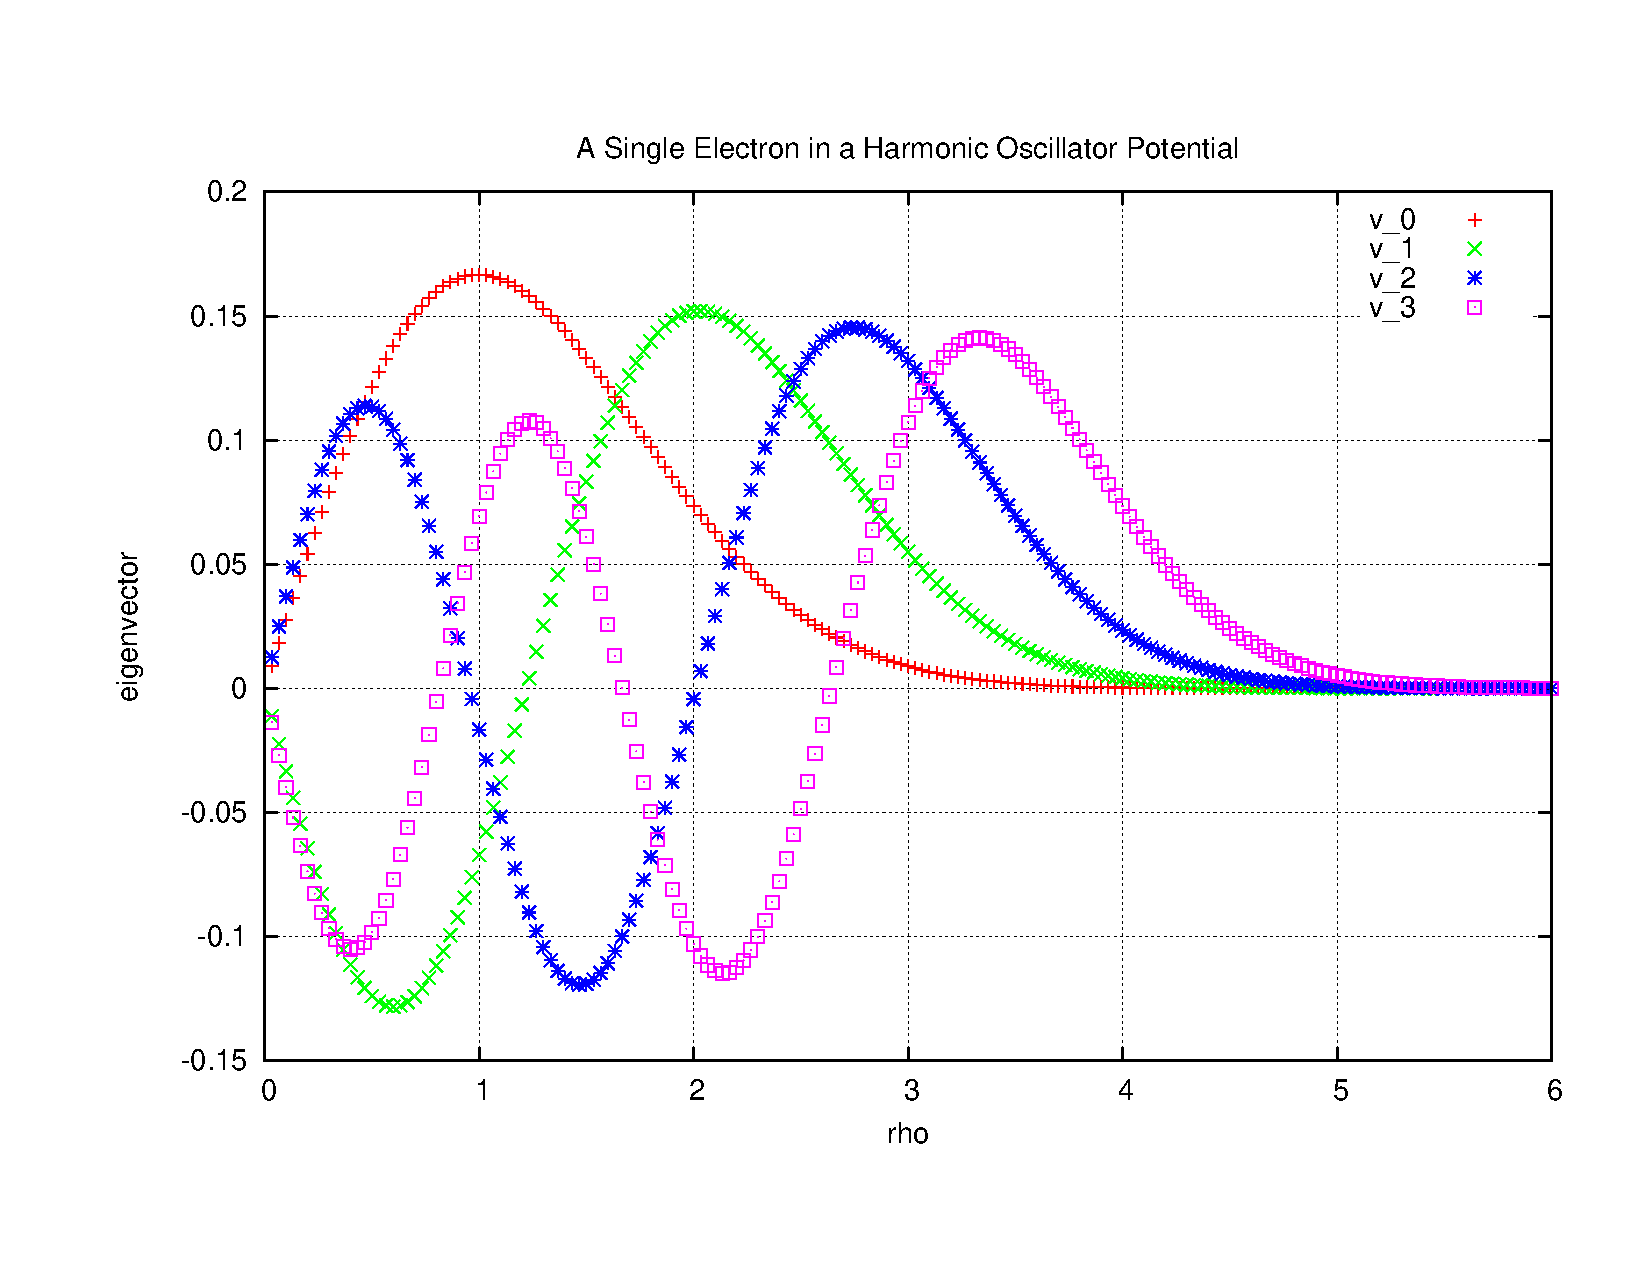
\includegraphics[width=1.0\textwidth]{1eHOcomparison.pdf}
\caption{Here we see a comparison of the lowest eigenvectors for a single electron a harmonic potential. Note that the numbering, 0, 1, 2, ..., is useful since it marks the number of nodes present within the specified eigenfunction. As the number increases, the function slowly moves farther away from the center.}
\end{figure}
\begin{figure}
\centering
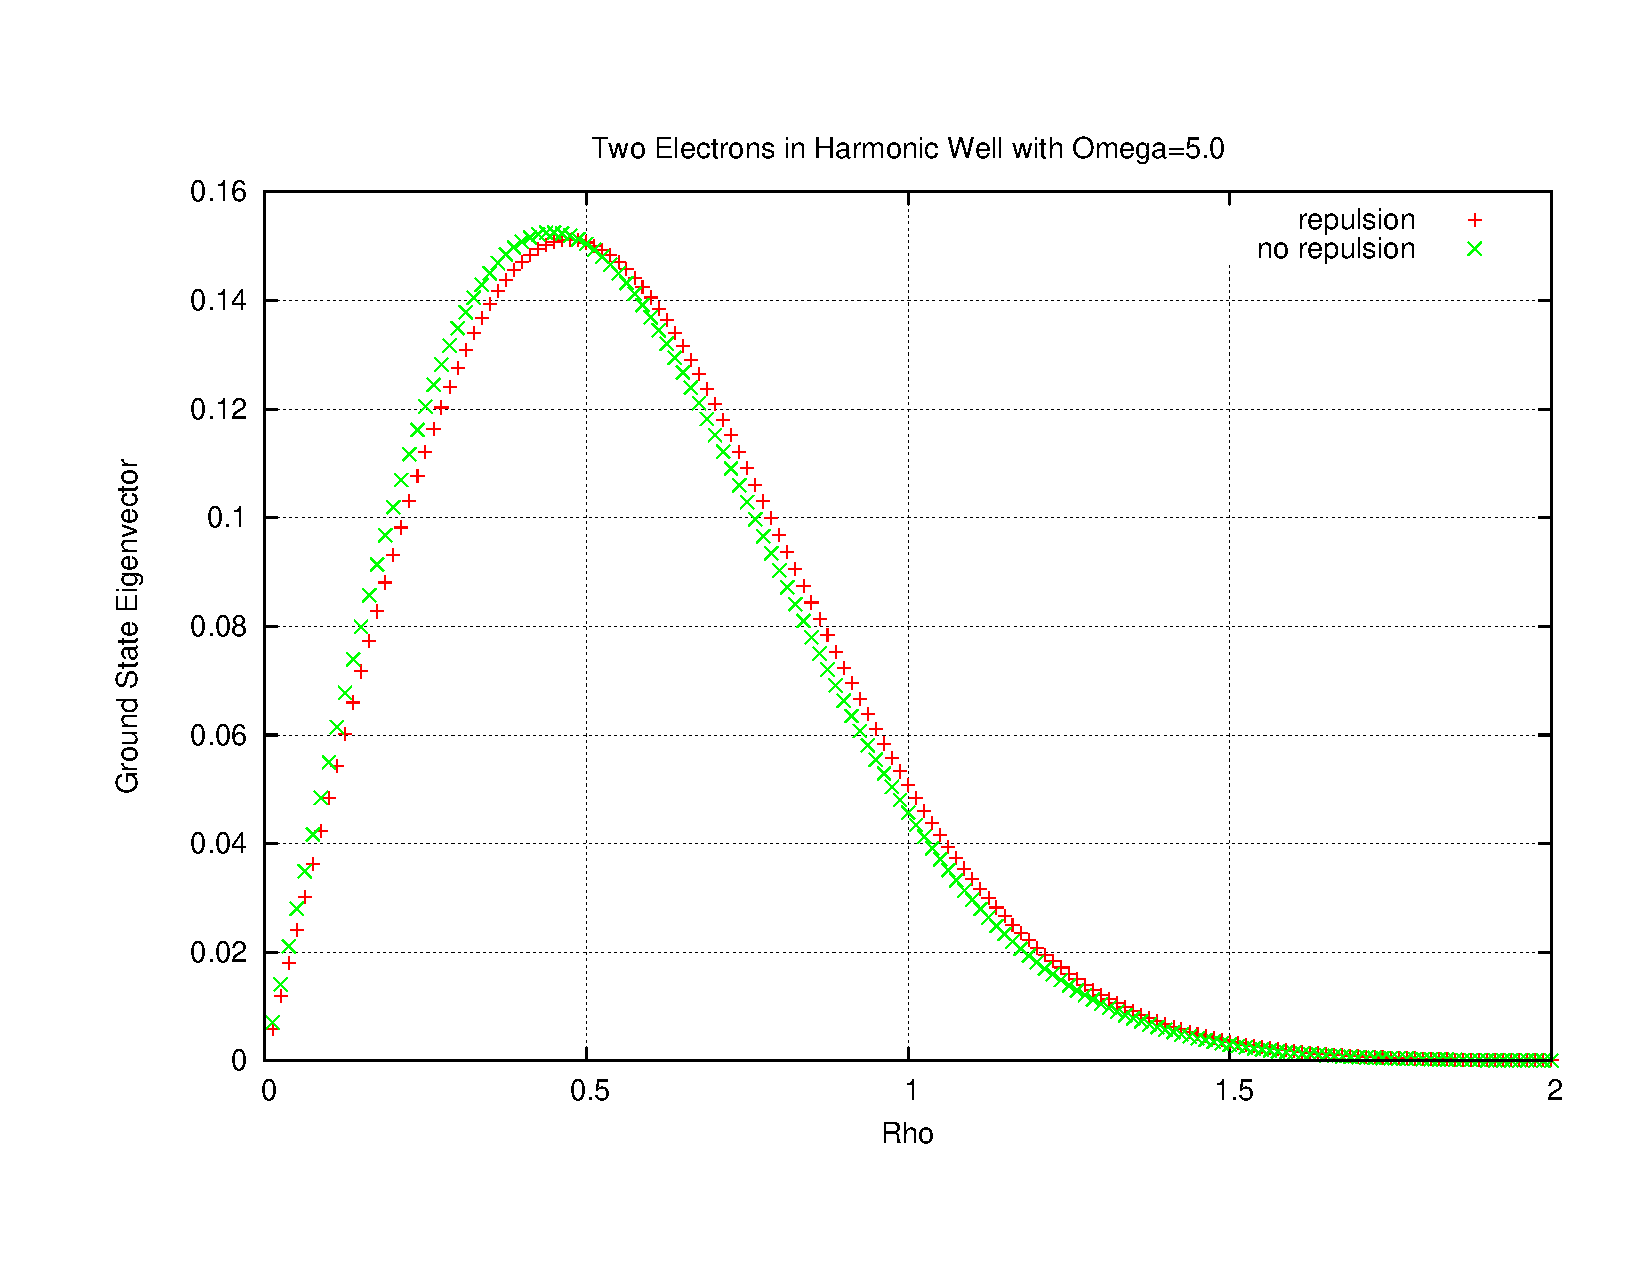
\includegraphics[width=1.0\textwidth]{2e_500.pdf}
\caption{Here we see a comparison of two electrons within a harmonic well, omega equal to 5.0. Note how the electrons are tightly bound when compared with the subsequent, lower values of omega. Additionally, though the cases of repulsion versus no repulsion are quite similar, we see that the with repulsion case is slightly farther out, as we'd expect. It is clear that repulsion plays a smaller role as the well becomes steeper.}
\end{figure}
\begin{figure}
\centering
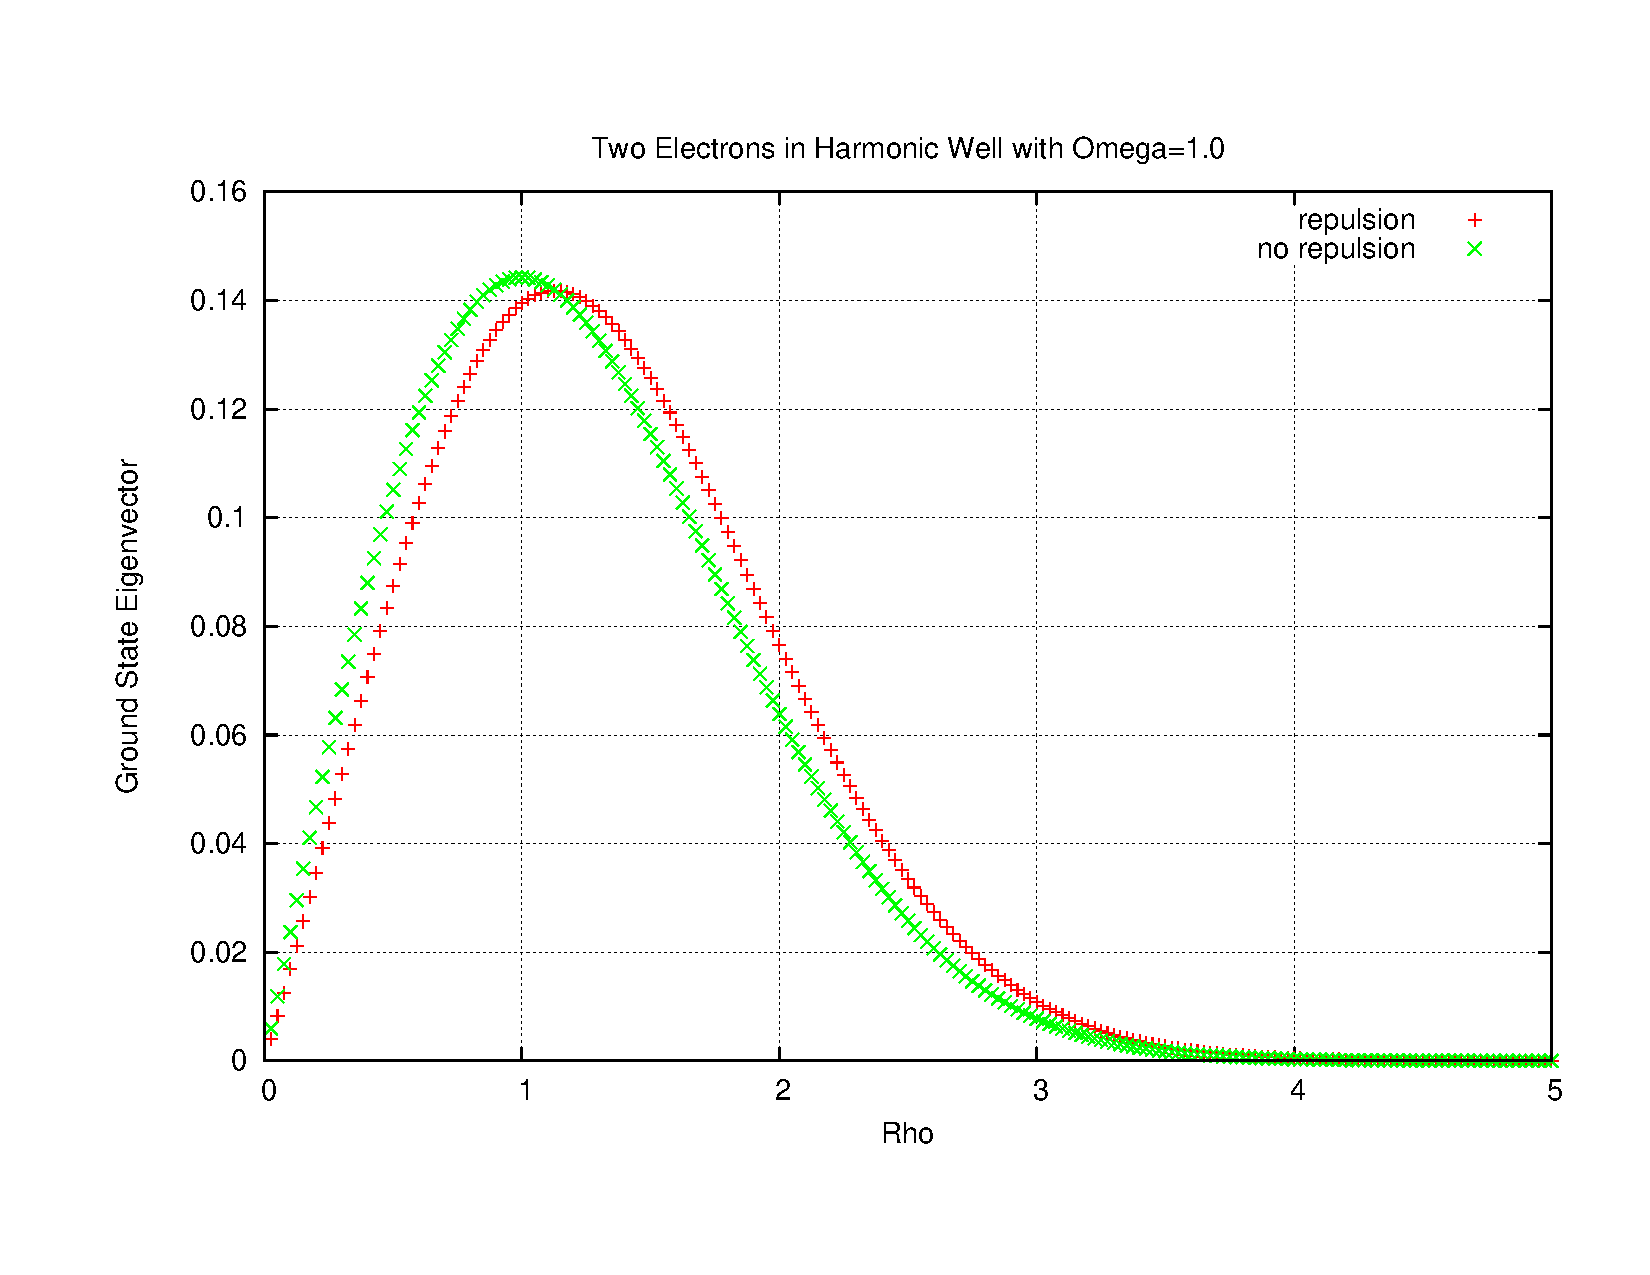
\includegraphics[width=1.0\textwidth]{2e_100.pdf}
\caption{Here we see a comparison of two electrons within a harmonic well, omega equal to 1.0. Note how the electrons have moved to slightly higher values of rho, and that the case with repulsion is now slightly more distrinct than with omega equal to 5.0. Again, it is farther out, account for the idea that repulsion "pushes" them farther apart.}
\end{figure}
\begin{figure}
\centering
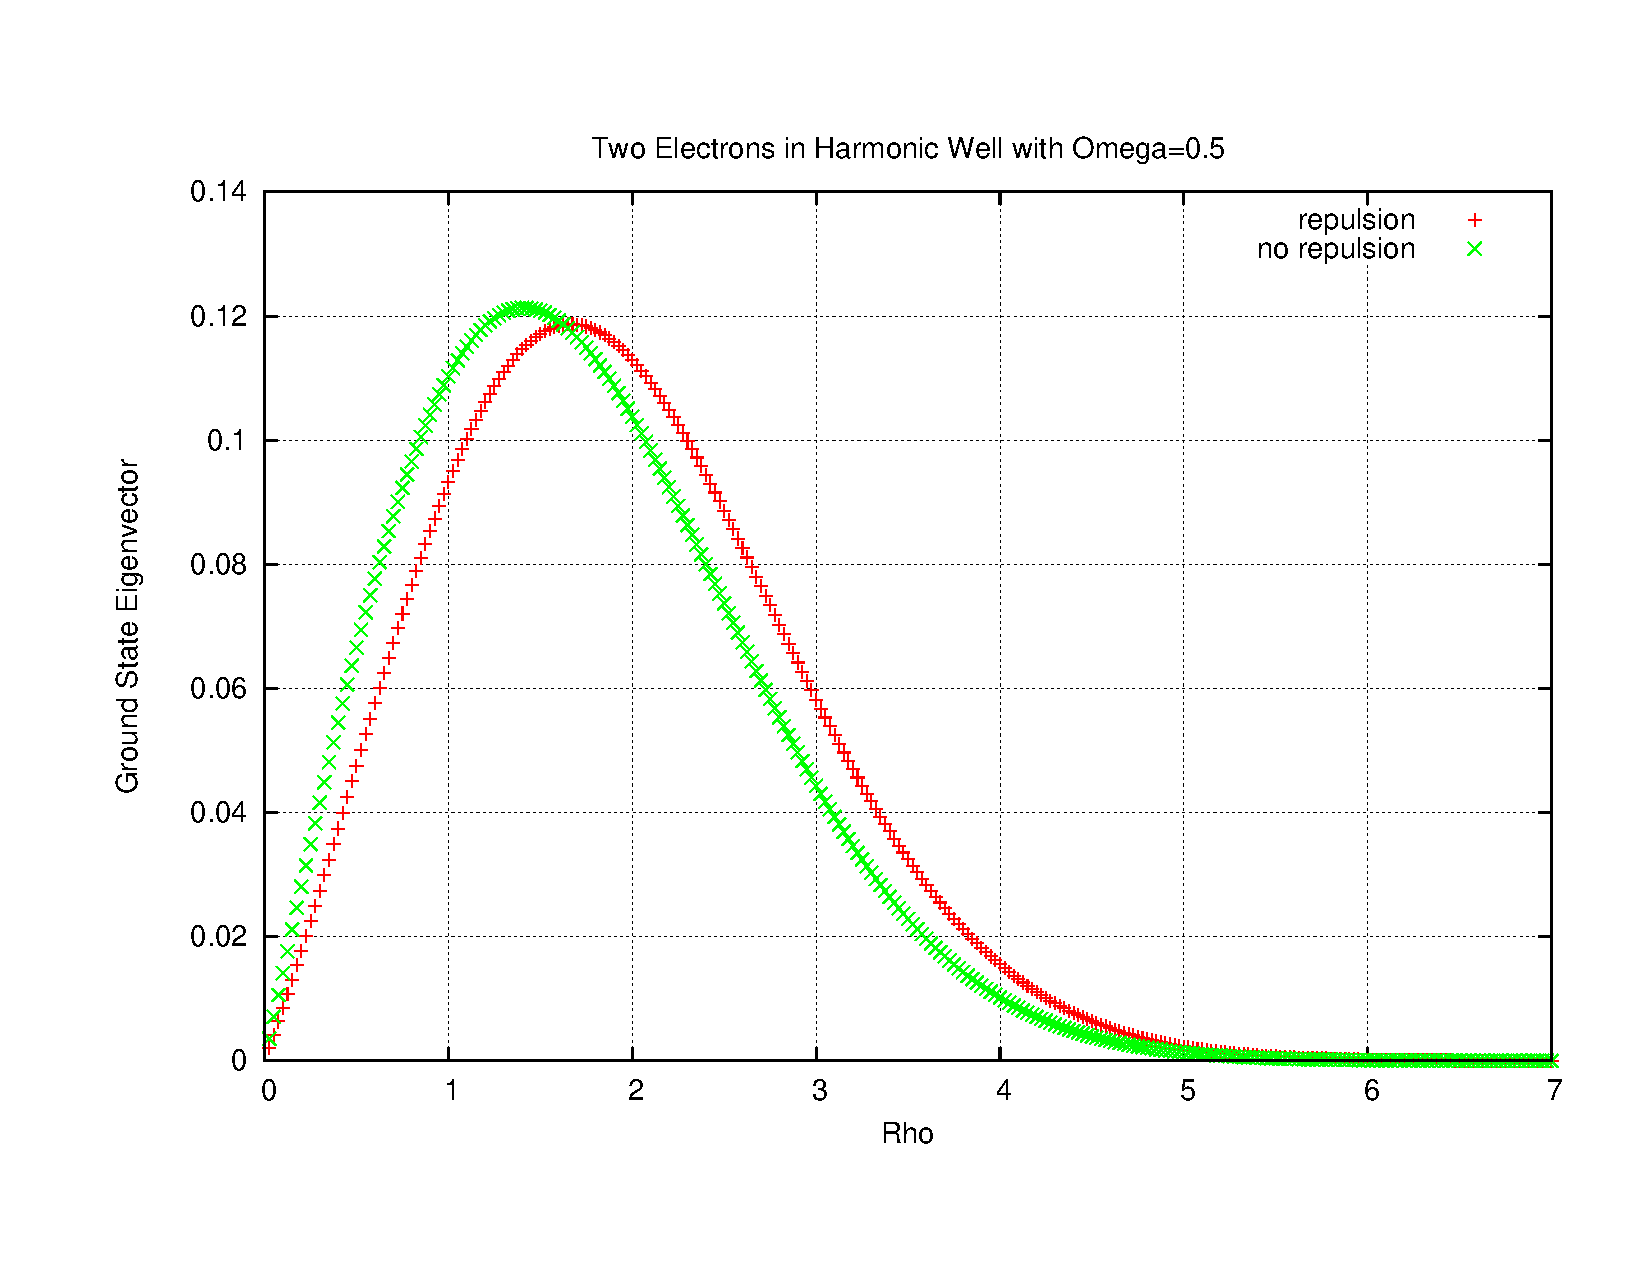
\includegraphics[width=1.0\textwidth]{2e_050.pdf}
\caption{Here we see a comparison of two electrons within a harmonic well, omega equal to 0.5. Note how the electrons have moved to larger values of rho, and that the case with repulsion is now even more distrinct than with omega equal to 5.0 or 1.0. It is once more farther out than the case of no repulsion.}
\end{figure}
\begin{figure}
\centering
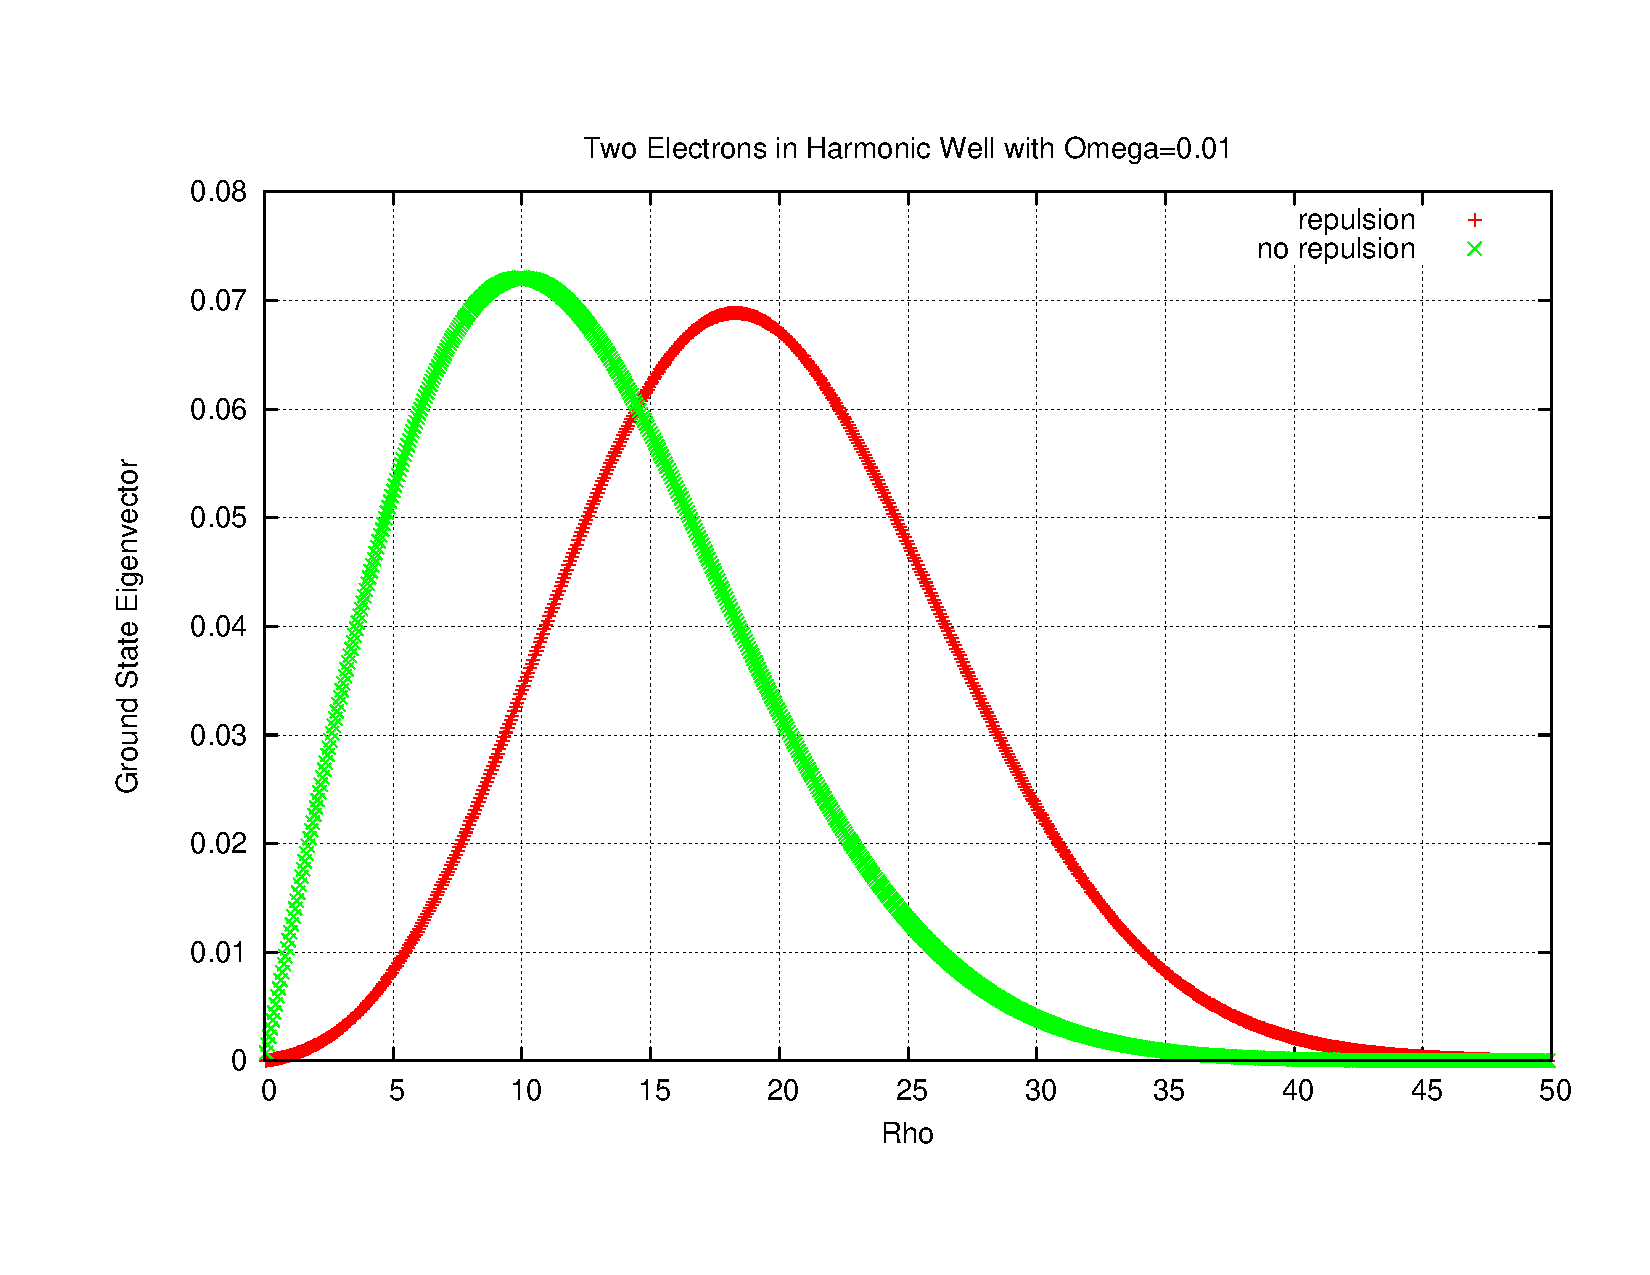
\includegraphics[width=1.0\textwidth]{2e_001.pdf}
\caption{Here we see a comparison of two electrons within a harmonic well, omega equal to 0.01. The electrons have now moved to significantly higher values of rho. The case of repulsion is even more separate from the case without and it is also farther from the center. As the well lessens, it is clear that repulsion plays a much larger role. As omega goes to zero, the electrons continue to move farther apart, to where omega is zero and they move to be infinitely far apart.}
\end{figure}
\section{Discussion}

Here we discuss both the computational accuracy, speed, and efficiency of Jacobi's algorithm and the comparison of two electrons with and without repulsion.

Jacobi's algorithm is certainly an accurate method for solving the eigenvalue problem, but it is a slow one for this particular problem. When compared with the armadillo eig-sys function, my eigensolver code was significantly slower, by 100-200 times. This is likely due to the fact that our selected hamiltonians were already tridiagonal, for which better algorithms exist and whose form Jacobi's algorithm readily destroys. 

In our selected cases, rho min was always selected to be zero, so we are left with variation in $\rho_{max}$ and matrix size as variable quantities. From figure (1) we see that increases in $n$ require substantial increases in the number of similarity rotations, scaling as 1.7-1.8$n^2$, which in turn lead to vast increases in computation time. From figure (2) we see that $\rho_{max}$ must be large enough so that the desired eigenvectors have gone to and will remain at zero; however, it must not be much larger, for increases in $\rho_{max}$ require increases in $n$ which lead to large computation times. Thus, we must be careful in our selection in our choice of both $\rho_{max}$ and $n$.

It is clear that the role of repulsion scales inversely with the strength of the potential, or with the value of omega. Repulsion plays a small role relative to the potential when omega is large and gains in importance as omega goes to zero, to the limiting case of omega equal to zero where repulsion would theoretically push the electrons to infinite separation distance. Figures (4)-(7) clearly show that the case of repulsion pushes the electrons farther apart, however slightly, for all cases when compared with no repulsion.

\section{Conclusion}

In this project we have investigated the use of Jacobi's algorithm as a method of solving the eigenvalue problem, specifically the case of electrons within a harmonic well. While the method is reliable given an appropriate matrix, it is computatonally intensive, requiring 1.7-1.8$n^2$ similarity rotations for a tridiagonal matrix, and lags significantly behind smarter algorithms, such as armadillo's eig-sys function, in our particular cases. It is clear that the inclusion of repulsion increases the mean sparation distance for the case of two electrons. Moreover, the degree to which the effect is significant is drastically affected by the strength of the potential well; steep potential wells reduce the influence of repulsion, whereas shallow wells allow for greater influence. 

\section{References}

[1] M. Hjorth-Jensen. Computational Physics, lecture notes spring 2016. Department of Physics, Michigan State University, 2016. \newline
[2] M. Taut. Nov 1993. Two electrons in an external oscillator potential: Particular analytical solutions of a Coulomb correlation problem. Phys. Rev. A. 48(5):3561-3566.

\newpage

\section*{Code Attachment}

\begin{lstlisting}[title={eigensolver.cpp}]
/********************************************************************
This code uses jacobi's algorithm to solve the eigenvalue problem.
Given an initial matrix, choice of orthonormal eigenvectors, matrix 
size, and tolerance for all offdiagonal matrix elements, the function 
jacobi_simrot_eigen_solver changes the given matrix to diagonal form
and the given eigenvectors to match the original matrix. 

The method uses a series of similarity rotations which zeros the
maximum element of the given matrix. After all off diagonal elements
are below the selected tolerance, we finish. The eigenvectors for the
original given matrix are reconstructed from the similarity rotations.
*********************************************************************/

#include<iostream>
#include<iomanip>
#include<cmath>
#include<fstream>
#include "time.h"

using namespace std;

//Function delcarations
void array_alloc(double*& a, int length);
void matrix_alloc(double**& A, int rows, int columns);
void array_delete(double*& a);
void matrix_delete(double**& A, int rows);
void symmat_offdiag_max(double**& A, int size, double& a_max, int& row, int& column);
void jacobi_simrot_eigen_solver(double**& A, double**& R, int size, double tolerance, int& count);
void array_print(double*& a, int length);
void matrix_print(double**& A, int rows, int columns);
void matrix_print_mult(double**& A, double**& B, int rowsA, int columnsA, int columnsB);
void matrix_diag_sort(double**& A, double**&B, int size);
void init_1eHO_matrices(double**& D, double**& R, int size, double rho_max, double rho_min);
void init_2eHO_matrices(double**& D, double**& R, int size, double rho_max, double rho_min, double omega);
void init_2eHOinter_matrices(double**& D, double**& R, int size, double rho_max, double rho_min, double omega);

//declare output file
ofstream ofile;

int main(int argc, char* argv[]){
	double** D, **R, **eigenvalues;
	char* outfilename;
	double h, rho_max, rho_min, omega, tolerance, time;
	int i, j, k, rows, columns, n, count;
	int eigvec_yesno, elecount, interacting;
	clock_t start, finish;
	tolerance = 1e-8;
	//Check proper entry arguments
	if(argc<9){
		cout << "Bad usage. Enter also 'outfilename rho_max rho_min matrix_size vectoroutput_1_0 electrons_2_1 interaction_1_0 omega' on same line." << endl;
		exit(1);
	}
	else{
		outfilename = argv[1];
		rho_max = atof(argv[2]);
		rho_min = atof(argv[3]);
		n = atoi(argv[4]);
		eigvec_yesno = atoi(argv[5]);
		elecount = atoi(argv[6]);
		interacting = atoi(argv[7]);
		omega = atof(argv[8]);	
		rows = n-2;
		columns = rows;
		h = (rho_max - rho_min)/((double) n);
	}
	//allocate matrices
	matrix_alloc(eigenvalues,rows,2);
	matrix_alloc(D, rows, columns);
	matrix_alloc(R, rows, columns);
	//Initialize matrices for selected conditions
	if(elecount==2){
		if(interacting==1){
			init_2eHOinter_matrices(D, R, rows, rho_max, rho_min, omega);
		}
		else if(interacting==0){
			init_2eHO_matrices(D, R, rows, rho_max, rho_min, omega);
		}
		else{
			cout << "Invalid entry for interaction choice. Please enter '1' for yes or '0' for no. Terminating..." << endl;
			exit(1);
		}
	}
	else if (elecount==1){
		init_1eHO_matrices(D, R, rows, rho_max, rho_min);
	}
	else{
		cout << "Invalid number of electrons. Enter '2' or '1'. Terminating..." << endl;
		exit(1);
	}
	//Conduct similarity rotations until all offdiag elements < tolerance.
	//Record time and number of similarity rotations.

	start = clock();
	jacobi_simrot_eigen_solver(D, R, rows, tolerance, count);
	finish = clock();
	time = ((finish-start)/(double) CLOCKS_PER_SEC);

	//Sort the eigenvalues from D from smallest to largest and note original positions
	//in order to retrieve constructed eigenvectors
	//Enter values in 'n' by '2' matrix, eigenvalues
	matrix_diag_sort(D, eigenvalues, rows);

	//Write output file
	ofile.open(outfilename);
	ofile.precision(7);
	if(eigvec_yesno==1){
		ofile << "#_i" << setw(15) << "eigenvalues" << setw(12) << "rho_i";
		for(i=0;i<rows;i++){
			ofile << setw(14) << "v_" << i;
		}
		ofile << endl;
		for(i=0;i<rows;i++){
			ofile << fixed << i << setw(15) << eigenvalues[i][0] << setw(15) << scientific << rho_min + h*(i+1);
			for(j=0;j<columns;j++){
				k=eigenvalues[j][1];
				ofile << setw(15) << R[i][k];
			}
			ofile << endl;
		}
	}
	else if(eigvec_yesno==0){
		ofile << "#_i" << setw(15) << "eigenvalues" << setw(15) << "j" << endl;
		for(i=0;i<rows;i++){
			ofile << i << setw(15) << eigenvalues[i][0] << setw(15) << eigenvalues[i][1] << endl;
		}
	}
	ofile.close();
	
	matrix_delete(eigenvalues,rows);
	matrix_delete(D,rows);
	matrix_delete(R,rows);
	

	//Print time and similarity rotations to screen
	cout << "\n\t" << count << " similarity rotations" << endl;
	cout << '\t' << time << " seconds" << endl << endl;

	return 0;
}


/******************************
Begin function definitions
*******************************/


void array_alloc(double*& a, int length){
	a = new double[length];
}
void matrix_alloc(double**& A, int rows, int columns){
	A = new double*[rows];
	for(int i=0;i<rows;i++){
		A[i] = new double[columns];
	}
}
void array_delete(double*& a){
	delete[] a;
}
void matrix_delete(double**& A, int rows){
	for(int i=0;i<rows;i++){
		delete[] A[i];
	}
	delete[] A;
}
//Old function to find max offdiagonal in symmetric matrix. No longer used.
void symmat_offdiag_max(double**& A, int size, double& a_max, int& row, int& column){
	double temp = 0.0;
	for(int i=0;i<size;i++){
		for(int j=i+1;j<size;j++){
			temp = fabs(A[i][j]);
			if(temp>a_max){
				a_max = temp;
				row = i;
				column = j;
			}
		}
	}
}
//Function to solve the eigenvalue problem given input matrix A, input orthonormal vectors R,
//size of the matrices, a tolerance for offdiagonal elements, and integer count for sim rot.
void jacobi_simrot_eigen_solver(double**& A, double**& R, int size, double tolerance, int& count){
	double a_ik, a_il, a_kk, a_ll, r_ik, r_il;
	double tau, tan, cos, sin;
	double temp, A_max;
	A_max = 0.0;
	int i, j, k, l;	
	//create array to find max element of each row in A and its column
	double** a_max = new double*[size];
	for(i=0;i<size;i++){
		a_max[i] = new double[2];
	}
	//initialize array so that any reference to improper value returns error
	for(i=0;i<size;i++){
		a_max[i][0] = 0;
		a_max[i][1] = -1;
	}
	//find max offdiagonal element of each row in A
	for(i=0;i<size;i++){
		for(j=i+1;j<size;j++){
			temp = fabs(A[i][j]);
			if(temp>a_max[i][0]){
				a_max[i][0] = temp;
				a_max[i][1] = j;
			}
		}
		if(a_max[i][0]>A_max){
			A_max = a_max[i][0];
			k = i;
			l = a_max[i][1];
		}
	}
	//set count of similarity rotations to zero for proper count
	count = 0;
	//conduct rotations until maximum offdiagonal in A is below tolerance
	while(A_max>tolerance){
		//calculate cos(theta) and sin(theta) from given offdiagonal
		tau = (A[l][l] - A[k][k])/(2*A[k][l]);
		if(tau>=0) tan = -tau + sqrt(tau*tau+1);
		else if(tau<0) tan = -tau - sqrt(tau*tau+1);
		cos = 1.0/sqrt(tan*tan + 1.0);
		sin = tan*cos;
		//calculate changes to A and R from rotation
		a_kk = A[k][k];
		a_ll = A[l][l];
		A[k][k] = a_kk*cos*cos + a_ll*sin*sin - 2.0*sin*cos*A[k][l];
		A[l][l] = a_kk*sin*sin + a_ll*cos*cos + 2.0*sin*cos*A[k][l];
		A[k][l] = 0.0;
		A[l][k] = 0.0;
		for(i=0;i<size;i++){
			if(i!=k && i!=l){
				a_ik = A[i][k];
				a_il = A[i][l];
				A[i][k] = a_ik*cos - a_il*sin;
				A[k][i] = A[i][k];
				A[i][l] = a_il*cos + a_ik*sin;
				A[l][i] = A[i][l];
			}
			r_ik = R[i][k];
			r_il = R[i][l];
			R[i][k] = r_ik*cos - r_il*sin;
			R[i][l] = r_ik*sin + r_il*cos;
		}

		//account for change to maximum element and to rows k and l.
		A_max = 0.0;
		a_max[k][0]=0.0;
		a_max[k][1]=-1;
		a_max[l][0]=0.0;
		a_max[l][1]=-1;

		//find new maximum elements for rows k and l
		for(j=k+1;j<size;j++){
			temp = fabs(A[k][j]);
			if(temp>a_max[k][0]){
				a_max[k][0] = temp;
				a_max[k][1] = j;
			}
		}
		for(j=l+1;j<size;j++){
			temp = fabs(A[l][j]);
			if(temp>a_max[l][0]){
				a_max[l][0] = temp;
				a_max[l][1] = j;
			}
		}
		//compare current maximum elements with changes in columns k and l
		for(i=0;i<k;i++){
			temp = fabs(A[i][k]);
			if(temp>a_max[i][0]){
				a_max[i][0] = temp;
				a_max[i][1] = k;
			}
		}
		for(i=0;i<l;i++){
			temp = fabs(A[i][l]);
			if(temp>a_max[i][0]){
				a_max[i][0] = temp;
				a_max[i][1] = l;
			}
		}	
		//find new maximum from array of maximum elements		
		for(i=0;i<size;i++){
			if(a_max[i][0]>A_max){
				A_max = a_max[i][0];
				k = i;
				l = a_max[i][1];
			}
		}
	//+1 similarity rotation
	count++;
	}
	//delete maximum array
	for(i=0;i<size;i++){
		delete[] a_max[i];
	}
	delete[] a_max;
}
void array_print(double*& a, int length){
	for(int i=0;i<length;i++){
		cout << a[i] << endl;
	}
}
void matrix_print(double**& A, int rows, int columns){
	for(int i=0;i<rows;i++){
		for(int j=0;j<columns;j++){
			cout << A[i][j] << '\t';
		}
		cout << '\n';
	}
}
void matrix_print_mult(double**& A, double**& B, int rowsA, int columnsA, int columnsB){
	double temp;	
	for(int i=0;i<rowsA;i++){
		for(int j=0;j<columnsB;j++){
			temp = 0.0;
			for(int p=0;p<columnsA;p++){
				temp += A[i][p]*B[p][j];
			}
			cout << temp << '\t';
		}
		cout << '\n';
	}
}
//sort diagonal elements of A into given 'size' by '2' matrix B, smallest to largest
void matrix_diag_sort(double**& A, double**&B, int size){
	int i, j, q;	
	for(i=0;i<size;i++){
		if(i==0){
			B[0][0]=A[0][0];
			B[0][1] = 0;
		}
		else{
			if(A[i][i]>=B[i-1][0]){
				B[i][0]=A[i][i];
				B[i][1]=i;
			}
			else{
				for(j=0;j<i;j++){
					if(A[i][i]<B[j][0]){
						for(q=i;q>j;q--){
							B[q][0] = B[q-1][0];
							B[q][1] = B[q-1][1];
						}
						B[j][0] = A[i][i];
						B[j][1] = i;
						break;
					}
				}
			}
		}
	}	
}
//initialize hamiltonian for one electron in harmonic well
void init_1eHO_matrices(double**& D, double**& R, int size, double rho_max, double rho_min){
	int i, j;	
	double rho, rho_sq, h, h_sq, temp1, temp2;
	h = (rho_max - rho_min)/((double) (size+1));
	h_sq = h*h;
	temp1 = 2.0/h_sq;
	temp2 = -1.0/h_sq;
	for(i=0;i<size;i++){
		rho = rho_min + (i+1)*h;
		rho_sq = rho*rho;
		for(j=0;j<size;j++){
			if(i==j){
				D[i][j] = temp1 + rho_sq;
				R[i][j] = 1.0;
			}
			else if(i==j+1||i==j-1){
				D[i][j] = temp2;
			}
			else{
				D[i][j] = 0.0;
				R[i][j] = 0.0;
			}
		}
	}	
}
//initialize hamiltonian for two electron in harmonic well, no interaction
void init_2eHO_matrices(double**& D, double**& R, int size, double rho_max, double rho_min, double omega){
	int i, j;	
	double rho, h, h_sq, temp1, temp2, omega_sq, potential;
	h = (rho_max - rho_min)/((double) (size+1));
	h_sq = h*h;
	omega_sq = omega*omega;
	temp1 = 2.0/h_sq;
	temp2 = -1.0/h_sq;
	for(i=0;i<size;i++){
		rho = rho_min + (i+1)*h;
		potential = omega_sq*rho*rho;
		for(j=0;j<size;j++){
			if(i==j){
				D[i][j] = temp1 + potential;
				R[i][j] = 1.0;
			}
			else if(i==j+1||i==j-1){
				D[i][j] = temp2;
			}
			else{
				D[i][j] = 0.0;
				R[i][j] = 0.0;
			}
		}
	}
}
//initialize hamiltonian for two electron in harmonic well, with interaction
void init_2eHOinter_matrices(double**& D, double**& R, int size, double rho_max, double rho_min, double omega){
	int i, j;	
	double rho, h, h_sq, temp1, temp2, omega_sq, potential;
	h = (rho_max - rho_min)/((double) (size+1));
	h_sq = h*h;
	omega_sq = omega*omega;
	temp1 = 2.0/h_sq;
	temp2 = -1.0/h_sq;
	for(i=0;i<size;i++){
		rho = rho_min + (i+1)*h;
		potential = omega_sq*rho*rho + 1.0/rho;
		for(j=0;j<size;j++){
			if(i==j){
				D[i][j] = temp1 + potential;
				R[i][j] = 1.0;
			}
			else if(i==j+1||i==j-1){
				D[i][j] = temp2;
			}
			else{
				D[i][j] = 0.0;
				R[i][j] = 0.0;
			}
		}
	}
}
\end{lstlisting}

\begin{lstlisting}[title={eigensolver-eigentime.cpp}]
/********************************************************************
This code adds to the eigensolver.cpp file. For further details, please
see annotation listed therein.

Additions include a loop over values of matrix size ranging from 20,
40, 60,...100, 200, ..., to 10^m, where m is input from the command
line execution. Two files are written. In each comparisons with 
armadillo's eig_sys function are included. One lists n, eigenvalues
from my code, eigenvalues from armadillo. The other lists n, n^2, sim
rot counts, my time, and arma's time. Note that one can still select
from the three cases, 1e, 2eNoI, 2eI.
*********************************************************************/

#include<iostream>
#include<iomanip>
#include<cmath>
#include<fstream>
#include "armadillo"
#include "time.h"

using namespace std;
using namespace arma;

void array_alloc(double*& a, int length);
void matrix_alloc(double**& A, int rows, int columns);
void array_delete(double*& a);
void matrix_delete(double**& A, int rows);
void symmat_offdiag_max(double**& A, int size, double& a_max, int& row, int& column);
void jacobi_simrot_eigen_solver(double**& A, double**& R, int size, double tolerance, int& count);
void array_print(double*& a, int length);
void matrix_print(double**& A, int rows, int columns);
void matrix_print_mult(double**& A, double**& B, int rowsA, int columnsA, int columnsB);
void matrix_diag_sort(double**& A, double**&B, int size);
void init_1eHO_matrices(double**& D, double**& R, int size, double rho_max, double rho_min);
void init_2eHO_matrices(double**& D, double**& R, int size, double rho_max, double rho_min, double omega);
void init_2eHOinter_matrices(double**& D, double**& R, int size, double rho_max, double rho_min, double omega);

//declare both out file streams
ofstream ofile, ofiletime;

int main(int argc, char* argv[]){
	double** D, **R, **eigenvalues;
	char* outfilename, *timefilename;
	double rho_max, rho_min, omega, tolerance, mytime, armatime;
	double rho, rho_sq, h, h_sq, temp1, temp2, potential, omega_sq;
	int p, q, m;
	int i, j, k, rows, columns, n, count;
	int eigvec_yesno, elecount, interacting;
	clock_t start, finish;
	tolerance = 1e-8;
//Check proper entry arguments
	if(argc<9){
		cout << "Bad usage. Enter also 'outfilename timefilename rho_max rho_min max_matrix_size electrons_2_1 interaction_1_0 omega' on same line." << endl;
		exit(1);
	}
	else{
		outfilename = argv[1];
		timefilename = argv[2];
		rho_max = atof(argv[3]);
		rho_min = atof(argv[4]);
	//Note that this input is the POWER of ten to which the loop will execute		
		m = atoi(argv[5]);
		elecount = atoi(argv[6]);
		interacting = atoi(argv[7]);
		omega = atof(argv[8]);
		omega_sq = omega*omega;
	}

//Open both out files
	ofile.open(outfilename);
	ofiletime.open(timefilename);
	ofile.precision(6);
	ofile << scientific;
	ofile << "#_n";
	for(i=0;i<5;i++){
		ofile << setw(15) << "eig_val_" << i;
	}
	for(i=0;i<5;i++){
		ofile << setw(15) << "eig_val_" << i;
	}
	ofile << endl;
	ofiletime << "#_n" << setw(15) << "n*n" << setw(15) << "sim rot" << setw(15) << "mytime" << setw(15) << "armatime" << endl;
//Conduct loops until 10^m	
	for(p=1;p<m;p++){
		for(q=2;q<11;q+=2){
			rows = q*pow(10.0,p);
			columns = rows;

			h = (rho_max - rho_min)/((double) (rows+1));
			h_sq = h*h;					
			temp1 = 2.0/h_sq;
			temp2 = -1.0/h_sq;

		//allocate matrices for my code and arma's code
			matrix_alloc(eigenvalues,rows,2);
			matrix_alloc(D, rows, columns);
			matrix_alloc(R, rows, columns);
			vec eig_a(rows);
			mat R_a(rows,rows);
			mat D_a(rows,rows);
		//Initialize matrices
			if(elecount==2){
				if(interacting==1){
					init_2eHOinter_matrices(D, R, rows, rho_max, rho_min, omega);	
					
					for(i=0;i<rows;i++){
						rho = rho_min + (i+1)*h;
						potential = omega_sq*rho*rho + 1.0/rho;
						for(j=0;j<rows;j++){
							if(i==j){
								D_a(i,j) = temp1 + potential;
								R_a(i,j) = 1.0;
							}
							else if(i==j+1||i==j-1){
								D_a(i,j) = temp2;
							}
							else{
								D_a(i,j) = 0.0;
								R_a(i,j) = 0.0;
							}
						}
					}
				}
				else if(interacting==0){
					init_2eHO_matrices(D, R, rows, rho_max, rho_min, omega);

					for(i=0;i<rows;i++){
						rho = rho_min + (i+1)*h;
						potential = omega_sq*rho*rho;
						for(j=0;j<rows;j++){
							if(i==j){
								D_a(i,j) = temp1 + potential;
								R_a(i,j) = 1.0;
							}
							else if(i==j+1||i==j-1){
								D_a(i,j) = temp2;
							}
							else{
								D_a(i,j) = 0.0;
								R_a(i,j) = 0.0;
							}
						}
					}
				}
				else{
					cout << "Invalid entry for interaction entry. Please enter '1' for yes or '0' for no. Terminating..." << endl;
				}
			}
			else if (elecount==1){
				init_1eHO_matrices(D, R, rows, rho_max, rho_min);

				for(i=0;i<rows;i++){
					rho = rho_min + (i+1)*h;
					rho_sq = rho*rho;
					for(j=0;j<rows;j++){
						if(i==j){
							D_a(i,j) = temp1 + rho_sq;
							R_a(i,j) = 1.0;
						}
						else if(i==j+1||i==j-1){
							D_a(i,j) = temp2;
						}
						else{
							D_a(i,j) = 0.0;
							R_a(i,j) = 0.0;
						}
					}
				}
			}
			else{
				cout << "Invalid number of electrons. Terminating..." << endl;
				exit(1);
			}
		
		//Conduct similarity rotations until all offdiag elements < tolerance
			start = clock();
			jacobi_simrot_eigen_solver(D, R, rows, tolerance, count);
			finish = clock();
			mytime = ((finish-start)/(double) CLOCKS_PER_SEC);

			start = clock();
			eig_sym(eig_a,R_a,D_a);
			finish = clock();
			armatime = ((finish-start)/(double) CLOCKS_PER_SEC);

		//Sort the eigenvalues from D from smallest to largest and note original positions
			matrix_diag_sort(D, eigenvalues, rows);

		//Write output file
			ofile << rows;
			for(i=0;i<5;i++){
				ofile << setw(15) << eigenvalues[i][0];
			}
			for(i=0;i<5;i++){
				ofile << setw(15) << eig_a[i];
			}
			ofile << endl;

			matrix_delete(eigenvalues,rows);
			matrix_delete(D,rows);
			matrix_delete(R,rows);

			ofiletime << rows << setw(15) << rows*rows << setw(15) << count << setw(15) << mytime << setw(15) << armatime << endl;

			cout << endl;
			cout << '\t' << rows << " matrix size" << endl;
			cout << '\t' << count << " similarity rotations" << endl;
			cout << '\t' << mytime << " seconds for my code" << endl;
			cout << '\t' << armatime << " seconds for armadillo" << endl;
		}
	}
	cout << endl;
	ofile.close();
	ofiletime.close();

	return 0;
}


/******************************
Begin function definitions
*******************************/


void array_alloc(double*& a, int length){
	a = new double[length];
}
void matrix_alloc(double**& A, int rows, int columns){
	A = new double*[rows];
	for(int i=0;i<rows;i++){
		A[i] = new double[columns];
	}
}
void array_delete(double*& a){
	delete[] a;
}
void matrix_delete(double**& A, int rows){
	for(int i=0;i<rows;i++){
		delete[] A[i];
	}
	delete[] A;
}
void symmat_offdiag_max(double**& A, int size, double& a_max, int& row, int& column){
	double temp = 0.0;
	for(int i=0;i<size;i++){
		for(int j=i+1;j<size;j++){
			temp = fabs(A[i][j]);
			if(temp>a_max){
				a_max = temp;
				row = i;
				column = j;
			}
		}
	}
}
void jacobi_simrot_eigen_solver(double**& A, double**& R, int size, double tolerance, int& count){
	double a_ik, a_il, a_kk, a_ll, r_ik, r_il;
	double tau, tan, cos, sin;
	double temp, A_max;
	A_max = 0.0;
	int i, j, k, l;	
	double** a_max = new double*[size];
	for(i=0;i<size;i++){
		a_max[i] = new double[2];
	}
	for(i=0;i<size;i++){
		a_max[i][0] = 0;
		a_max[i][1] = -1;
	}
	for(i=0;i<size;i++){
		for(j=i+1;j<size;j++){
			temp = fabs(A[i][j]);
			if(temp>a_max[i][0]){
				a_max[i][0] = temp;
				a_max[i][1] = j;
			}
		}
		if(a_max[i][0]>A_max){
			A_max = a_max[i][0];
			k = i;
			l = a_max[i][1];
		}
	}
	count = 0;
	while(A_max>tolerance){
		tau = (A[l][l] - A[k][k])/(2*A[k][l]);
		if(tau>=0) tan = -tau + sqrt(tau*tau+1);
		else if(tau<0) tan = -tau - sqrt(tau*tau+1);
		cos = 1.0/sqrt(tan*tan + 1.0);
		sin = tan*cos;

		a_kk = A[k][k];
		a_ll = A[l][l];
		A[k][k] = a_kk*cos*cos + a_ll*sin*sin - 2.0*sin*cos*A[k][l];
		A[l][l] = a_kk*sin*sin + a_ll*cos*cos + 2.0*sin*cos*A[k][l];
		A[k][l] = 0.0;
		A[l][k] = 0.0;
		for(i=0;i<size;i++){
			if(i!=k && i!=l){
				a_ik = A[i][k];
				a_il = A[i][l];
				A[i][k] = a_ik*cos - a_il*sin;
				A[k][i] = A[i][k];
				A[i][l] = a_il*cos + a_ik*sin;
				A[l][i] = A[i][l];
			}
			r_ik = R[i][k];
			r_il = R[i][l];
			R[i][k] = r_ik*cos - r_il*sin;
			R[i][l] = r_ik*sin + r_il*cos;
		}

	
		A_max = 0.0;
		a_max[k][0]=0.0;
		a_max[k][1]=-1;
		a_max[l][0]=0.0;
		a_max[l][1]=-1;

		for(j=k+1;j<size;j++){
			temp = fabs(A[k][j]);
			if(temp>a_max[k][0]){
				a_max[k][0] = temp;
				a_max[k][1] = j;
			}
		}
		for(j=l+1;j<size;j++){
			temp = fabs(A[l][j]);
			if(temp>a_max[l][0]){
				a_max[l][0] = temp;
				a_max[l][1] = j;
			}
		}
		for(i=0;i<k;i++){
			temp = fabs(A[i][k]);
			if(temp>a_max[i][0]){
				a_max[i][0] = temp;
				a_max[i][1] = k;
			}
		}
		for(i=0;i<l;i++){
			temp = fabs(A[i][l]);
			if(temp>a_max[i][0]){
				a_max[i][0] = temp;
				a_max[i][1] = l;
			}
		}			
		for(i=0;i<size;i++){
			if(a_max[i][0]>A_max){
				A_max = a_max[i][0];
				k = i;
				l = a_max[i][1];
			}
		}
	count++;
	}

	for(i=0;i<size;i++){
		delete[] a_max[i];
	}
	delete[] a_max;
}
void array_print(double*& a, int length){
	for(int i=0;i<length;i++){
		cout << a[i] << endl;
	}
}
void matrix_print(double**& A, int rows, int columns){
	for(int i=0;i<rows;i++){
		for(int j=0;j<columns;j++){
			cout << A[i][j] << '\t';
		}
		cout << '\n';
	}
}
void matrix_print_mult(double**& A, double**& B, int rowsA, int columnsA, int columnsB){
	double temp;	
	for(int i=0;i<rowsA;i++){
		for(int j=0;j<columnsB;j++){
			temp = 0.0;
			for(int p=0;p<columnsA;p++){
				temp += A[i][p]*B[p][j];
			}
			cout << temp << '\t';
		}
		cout << '\n';
	}
}
void matrix_diag_sort(double**& A, double**&B, int size){
	int i, j, q;	
	for(i=0;i<size;i++){
		if(i==0){
			B[0][0]=A[0][0];
			B[0][1] = 0;
		}
		else{
			if(A[i][i]>=B[i-1][0]){
				B[i][0]=A[i][i];
				B[i][1]=i;
			}
			else{
				for(j=0;j<i;j++){
					if(A[i][i]<B[j][0]){
						for(q=i;q>j;q--){
							B[q][0] = B[q-1][0];
							B[q][1] = B[q-1][1];
						}
						B[j][0] = A[i][i];
						B[j][1] = i;
						break;
					}
				}
			}
		}
	}	
}
void init_1eHO_matrices(double**& D, double**& R, int size, double rho_max, double rho_min){
	int i, j;	
	double rho, rho_sq, h, h_sq, temp1, temp2;
	h = (rho_max - rho_min)/((double) (size+1));
	h_sq = h*h;
	temp1 = 2.0/h_sq;
	temp2 = -1.0/h_sq;
	for(i=0;i<size;i++){
		rho = rho_min + (i+1)*h;
		rho_sq = rho*rho;
		for(j=0;j<size;j++){
			if(i==j){
				D[i][j] = temp1 + rho_sq;
				R[i][j] = 1.0;
			}
			else if(i==j+1||i==j-1){
				D[i][j] = temp2;
			}
			else{
				D[i][j] = 0.0;
				R[i][j] = 0.0;
			}
		}
	}	
}
void init_2eHO_matrices(double**& D, double**& R, int size, double rho_max, double rho_min, double omega){
	int i, j;	
	double rho, h, h_sq, temp1, temp2, omega_sq, potential;
	h = (rho_max - rho_min)/((double) (size+1));
	h_sq = h*h;
	omega_sq = omega*omega;
	temp1 = 2.0/h_sq;
	temp2 = -1.0/h_sq;
	for(i=0;i<size;i++){
		rho = rho_min + (i+1)*h;
		potential = omega_sq*rho*rho;
		for(j=0;j<size;j++){
			if(i==j){
				D[i][j] = temp1 + potential;
				R[i][j] = 1.0;
			}
			else if(i==j+1||i==j-1){
				D[i][j] = temp2;
			}
			else{
				D[i][j] = 0.0;
				R[i][j] = 0.0;
			}
		}
	}
}
void init_2eHOinter_matrices(double**& D, double**& R, int size, double rho_max, double rho_min, double omega){
	int i, j;	
	double rho, h, h_sq, temp1, temp2, omega_sq, potential;
	h = (rho_max - rho_min)/((double) (size+1));
	h_sq = h*h;
	omega_sq = omega*omega;
	temp1 = 2.0/h_sq;
	temp2 = -1.0/h_sq;
	for(i=0;i<size;i++){
		rho = rho_min + (i+1)*h;
		potential = omega_sq*rho*rho + 1.0/rho;
		for(j=0;j<size;j++){
			if(i==j){
				D[i][j] = temp1 + potential;
				R[i][j] = 1.0;
			}
			else if(i==j+1||i==j-1){
				D[i][j] = temp2;
			}
			else{
				D[i][j] = 0.0;
				R[i][j] = 0.0;
			}
		}
	}
}
\end{lstlisting}
\begin{lstlisting}[title={eigensolver-unittest.cpp}]
/********************************************************************
This code reads as eigensolver.cpp. For further details please read
annotations therein.

Additions here include unit tests for consistent orthonormality
throughout the entirety of the similarity rotations. Additional unit
tests could include tests of the sorting algorithm, the eigen solver
results, and so forth. These have been tested visually against multiple 
analytical solutions, but no code has been written for this purpose. 
*********************************************************************/

#include<iostream>
#include<iomanip>
#include<cmath>
#include<fstream>
#include "time.h"
#include "stdlib.h"

using namespace std;

void array_alloc(double*& a, int length);
void matrix_alloc(double**& A, int rows, int columns);
void array_delete(double*& a);
void matrix_delete(double**& A, int rows);
void symmat_offdiag_max(double**& A, int size, double& a_max, int& row, int& column);
void jacobi_simrot_eigen_solver(double**& A, double**& R, int size, double tolerance, int& count);
void array_print(double*& a, int length);
void matrix_print(double**& A, int rows, int columns);
void matrix_print_mult(double**& A, double**& B, int rowsA, int columnsA, int columnsB);
void matrix_diag_sort(double**& A, double**&B, int size);
void init_1eHO_matrices(double**& D, double**& R, int size, double rho_max, double rho_min);
void init_2eHO_matrices(double**& D, double**& R, int size, double rho_max, double rho_min, double omega);
void init_2eHOinter_matrices(double**& D, double**& R, int size, double rho_max, double rho_min, double omega);

ofstream ofile;

int main(int argc, char* argv[]){
	double** D, **R, **eigenvalues;
	char* outfilename;
	double h, rho_max, rho_min, omega, tolerance, time;
	int i, j, k, rows, columns, n, count;
	int eigvec_yesno, elecount, interacting;
	clock_t start, finish;
	tolerance = 1e-10;
//Check proper entry arguments
	if(argc<9){
		cout << "Bad usage. Enter also 'outfilename rho_max rho_min matrix_size vectoroutput_1_0 electrons_2_1 interaction_1_0 omega' on same line." << endl;
		exit(1);
	}
	else{
		outfilename = argv[1];
		rho_max = atof(argv[2]);
		rho_min = atof(argv[3]);
		n = atoi(argv[4]);
		eigvec_yesno = atoi(argv[5]);
		elecount = atoi(argv[6]);
		interacting = atoi(argv[7]);
		omega = atof(argv[8]);	
		rows = n;
		columns = rows;
		h = (rho_max - rho_min)/((double) n+2);
	}
//allocate matrices
	matrix_alloc(eigenvalues,rows,2);
	matrix_alloc(D, rows, columns);
	matrix_alloc(R, rows, columns);
//Initialize matrices
	if(elecount==2){
		if(interacting==1){
			init_2eHOinter_matrices(D, R, rows, rho_max, rho_min, omega);
		}
		else if(interacting==0){
			init_2eHO_matrices(D, R, rows, rho_max, rho_min, omega);
		}
		else{
			cout << "Invalid entry for interaction entry. Please enter '1' for yes or '0' for no. Terminating..." << endl;
		}
	}
	else if (elecount==1){
		init_1eHO_matrices(D, R, rows, rho_max, rho_min);
	}
	else{
		cout << "Invalid number of electrons. Terminating..." << endl;
		exit(1);
	}
//Conduct similarity rotations until all offdiag elements < tolerance

	start = clock();
	jacobi_simrot_eigen_solver(D, R, rows, tolerance, count);
	finish = clock();
	time = ((finish-start)/(double) CLOCKS_PER_SEC);

//Sort the eigenvalues from D from smallest to largest and note original positions
	matrix_diag_sort(D, eigenvalues, rows);

//Write output file
	ofile.open(outfilename);
	ofile.precision(4);
	if(eigvec_yesno==1){
		ofile << "#_i" << setw(15) << "eigenvalues" << setw(12) << "rho_i";
		for(i=0;i<rows;i++){
			ofile << setw(14) << "v_" << i;
		}
		ofile << endl;
		for(i=0;i<rows;i++){
			ofile << fixed << i << setw(15) << eigenvalues[i][0] << setw(15) << scientific << rho_min + h*(i+1);
			for(j=0;j<columns;j++){
				k=eigenvalues[j][1];
				ofile << setw(15) << R[i][k];
			}
			ofile << endl;
		}
	}
	else if(eigvec_yesno==0){
		ofile << "#_i" << setw(15) << "eigenvalues" << setw(15) << "j" << endl;
		for(i=0;i<rows;i++){
			ofile << i << setw(15) << eigenvalues[i][0] << setw(15) << eigenvalues[i][1] << endl;
		}
	}
	ofile.close();
	
	matrix_delete(eigenvalues,rows);
	matrix_delete(D,rows);
	matrix_delete(R,rows);
	
	cout << '\t' << count << " similarity rotations" << endl;
	cout << '\t' << time << " seconds" << endl;

	return 0;
}


/******************************
Begin function definitions
*******************************/


void array_alloc(double*& a, int length){
	a = new double[length];
}
void matrix_alloc(double**& A, int rows, int columns){
	A = new double*[rows];
	for(int i=0;i<rows;i++){
		A[i] = new double[columns];
	}
}
void array_delete(double*& a){
	delete[] a;
}
void matrix_delete(double**& A, int rows){
	for(int i=0;i<rows;i++){
		delete[] A[i];
	}
	delete[] A;
}
void symmat_offdiag_max(double**& A, int size, double& a_max, int& row, int& column){
	double temp = 0.0;
	for(int i=0;i<size;i++){
		for(int j=i+1;j<size;j++){
			temp = fabs(A[i][j]);
			if(temp>a_max){
				a_max = temp;
				row = i;
				column = j;
			}
		}
	}
}
void jacobi_simrot_eigen_solver(double**& A, double**& R, int size, double tolerance, int& count){
	double a_ik, a_il, a_kk, a_ll, r_ik, r_il;
	double tau, tan, cos, sin;
	double temp, A_max;
	double unit_test, unit_test1, unit_test2, unit_tolerance;
	int r1, r2;
	int i, j, k, l;	
	srand(time(NULL));
	A_max = 0.0;
	unit_tolerance = tolerance;
	double** a_max = new double*[size];
	for(i=0;i<size;i++){
		a_max[i] = new double[2];
	}
	for(i=0;i<size;i++){
		a_max[i][0] = 0;
		a_max[i][1] = -1;
	}
	for(i=0;i<size;i++){
		for(j=i+1;j<size;j++){
			temp = fabs(A[i][j]);
			if(temp>a_max[i][0]){
				a_max[i][0] = temp;
				a_max[i][1] = j;
			}
		}
		if(a_max[i][0]>A_max){
			A_max = a_max[i][0];
			k = i;
			l = a_max[i][1];
		}
	}
	count = 0;
	while(A_max>tolerance){
		count++;		
		tau = (A[l][l] - A[k][k])/(2*A[k][l]);
		if(tau>=0) tan = -tau + sqrt(tau*tau+1);
		else if(tau<0) tan = -tau - sqrt(tau*tau+1);
		cos = 1.0/sqrt(tan*tan + 1.0);
		sin = tan*cos;

		a_kk = A[k][k];
		a_ll = A[l][l];
		A[k][k] = a_kk*cos*cos + a_ll*sin*sin - 2.0*sin*cos*A[k][l];
		A[l][l] = a_kk*sin*sin + a_ll*cos*cos + 2.0*sin*cos*A[k][l];
		A[k][l] = 0.0;
		A[l][k] = 0.0;
		for(i=0;i<size;i++){
			if(i!=k && i!=l){
				a_ik = A[i][k];
				a_il = A[i][l];
				A[i][k] = a_ik*cos - a_il*sin;
				A[k][i] = A[i][k];
				A[i][l] = a_il*cos + a_ik*sin;
				A[l][i] = A[i][l];
			}
			r_ik = R[i][k];
			r_il = R[i][l];
			R[i][k] = r_ik*cos - r_il*sin;
			R[i][l] = r_ik*sin + r_il*cos;
		}
/*****************************
Orthonormality unit test for 
random eigenvectors r1, r2
******************************/
		if(count%10==0){
			unit_test = 0.0;
			r1 = rand()%size;
			r2 = rand()%size;
			while(r1==r2){
				r2 = rand()%size;
			}
			for(i=0;i<size;i++){
				unit_test += (R[i][r1])*(R[i][r2]);
			}
			if(unit_test>unit_tolerance||unit_test<-unit_tolerance){
				cout << "Orthogonality test failed on similarity rotation " << count << " for vectors " << r1 << " and " << r2 << endl;
				cout << "Terminating program..." << endl;
				exit(1);
			}

			unit_test1 = 0.0; unit_test2 = 0.0;
			for(i=0;i<size;i++){
				unit_test1 += R[i][r1]*R[i][r1];
				unit_test2 += R[i][r2]*R[i][r2];
			}
			if(unit_test1>1+unit_tolerance||unit_test1<1-unit_tolerance){
				cout << "Normality test failed on similarity rotation " << count << " for vector "<< r1 << endl;
				cout << "Terminating program..." << endl;
				exit(1);			
			}
			if(unit_test2>1+unit_tolerance||unit_test2<1-unit_tolerance){
				cout << "Normality test failed on similarity rotation " << count << " for vector " << r2 << endl;			
				cout << "Terminating program..." << endl;
				exit(1);			
			}
		}
/*****************************
End orthonormality unit test
******************************/
		A_max = 0.0;
		a_max[k][0]=0.0;
		a_max[k][1]=-1;
		a_max[l][0]=0.0;
		a_max[l][1]=-1;

		for(j=k+1;j<size;j++){
			temp = fabs(A[k][j]);
			if(temp>a_max[k][0]){
				a_max[k][0] = temp;
				a_max[k][1] = j;
			}
		}
		for(j=l+1;j<size;j++){
			temp = fabs(A[l][j]);
			if(temp>a_max[l][0]){
				a_max[l][0] = temp;
				a_max[l][1] = j;
			}
		}
		for(i=0;i<k;i++){
			temp = fabs(A[i][k]);
			if(temp>a_max[i][0]){
				a_max[i][0] = temp;
				a_max[i][1] = k;
			}
		}
		for(i=0;i<l;i++){
			temp = fabs(A[i][l]);
			if(temp>a_max[i][0]){
				a_max[i][0] = temp;
				a_max[i][1] = l;
			}
		}			
		for(i=0;i<size;i++){
			if(a_max[i][0]>A_max){
				A_max = a_max[i][0];
				k = i;
				l = a_max[i][1];
			}
		}
	}

	
			

	for(i=0;i<size;i++){
		delete[] a_max[i];
	}
	delete[] a_max;
}
void array_print(double*& a, int length){
	for(int i=0;i<length;i++){
		cout << a[i] << endl;
	}
}
void matrix_print(double**& A, int rows, int columns){
	for(int i=0;i<rows;i++){
		for(int j=0;j<columns;j++){
			cout << A[i][j] << '\t';
		}
		cout << '\n';
	}
}
void matrix_print_mult(double**& A, double**& B, int rowsA, int columnsA, int columnsB){
	double temp;	
	for(int i=0;i<rowsA;i++){
		for(int j=0;j<columnsB;j++){
			temp = 0.0;
			for(int p=0;p<columnsA;p++){
				temp += A[i][p]*B[p][j];
			}
			cout << temp << '\t';
		}
		cout << '\n';
	}
}
void matrix_diag_sort(double**& A, double**&B, int size){
	int i, j, q;	
	for(i=0;i<size;i++){
		if(i==0){
			B[0][0]=A[0][0];
			B[0][1] = 0;
		}
		else{
			if(A[i][i]>=B[i-1][0]){
				B[i][0]=A[i][i];
				B[i][1]=i;
			}
			else{
				for(j=0;j<i;j++){
					if(A[i][i]<B[j][0]){
						for(q=i;q>j;q--){
							B[q][0] = B[q-1][0];
							B[q][1] = B[q-1][1];
						}
						B[j][0] = A[i][i];
						B[j][1] = i;
						break;
					}
				}
			}
		}
	}	
}
void init_1eHO_matrices(double**& D, double**& R, int size, double rho_max, double rho_min){
	int i, j;	
	double rho, rho_sq, h, h_sq, temp1, temp2;
	h = (rho_max - rho_min)/((double) (size+1));
	h_sq = h*h;
	temp1 = 2.0/h_sq;
	temp2 = -1.0/h_sq;
	for(i=0;i<size;i++){
		rho = rho_min + (i+1)*h;
		rho_sq = rho*rho;
		for(j=0;j<size;j++){
			if(i==j){
				D[i][j] = temp1 + rho_sq;
				R[i][j] = 1.0;
			}
			else if(i==j+1||i==j-1){
				D[i][j] = temp2;
			}
			else{
				D[i][j] = 0.0;
				R[i][j] = 0.0;
			}
		}
	}	
}
void init_2eHO_matrices(double**& D, double**& R, int size, double rho_max, double rho_min, double omega){
	int i, j;	
	double rho, h, h_sq, temp1, temp2, omega_sq, potential;
	h = (rho_max - rho_min)/((double) (size+1));
	h_sq = h*h;
	omega_sq = omega*omega;
	temp1 = 2.0/h_sq;
	temp2 = -1.0/h_sq;
	for(i=0;i<size;i++){
		rho = rho_min + (i+1)*h;
		potential = omega_sq*rho*rho;
		for(j=0;j<size;j++){
			if(i==j){
				D[i][j] = temp1 + potential;
				R[i][j] = 1.0;
			}
			else if(i==j+1||i==j-1){
				D[i][j] = temp2;
			}
			else{
				D[i][j] = 0.0;
				R[i][j] = 0.0;
			}
		}
	}
}
void init_2eHOinter_matrices(double**& D, double**& R, int size, double rho_max, double rho_min, double omega){
	int i, j;	
	double rho, h, h_sq, temp1, temp2, omega_sq, potential;
	h = (rho_max - rho_min)/((double) (size+1));
	h_sq = h*h;
	omega_sq = omega*omega;
	temp1 = 2.0/h_sq;
	temp2 = -1.0/h_sq;
	for(i=0;i<size;i++){
		rho = rho_min + (i+1)*h;
		potential = omega_sq*rho*rho + 1.0/rho;
		for(j=0;j<size;j++){
			if(i==j){
				D[i][j] = temp1 + potential;
				R[i][j] = 1.0;
			}
			else if(i==j+1||i==j-1){
				D[i][j] = temp2;
			}
			else{
				D[i][j] = 0.0;
				R[i][j] = 0.0;
			}
		}
	}
}
\end{lstlisting}
\end{document}


